\documentclass[12pt,twoside]{report}
% \usepackage{fontspec}

\usepackage{tabularx}
\usepackage{tikz}
\usetikzlibrary{positioning, fit, arrows.meta}
\usepackage{amsmath,amssymb}

% \setmonofont{Inconsolata}
\usepackage{listings}
\usepackage{color}
\usepackage{xcolor}
\usepackage{algorithm}
\usepackage[noend]{algpseudocode}
\makeatletter
\def\BState{\State\hskip-\ALG@thistlm}
\makeatother
 
\definecolor{codegreen}{rgb}{0,0.6,0}
\definecolor{codegray}{rgb}{0.5,0.5,0.5}
\definecolor{codepurple}{rgb}{0.58,0,0.82}
\definecolor{backcolour}{rgb}{0.95,0.95,0.92}
 
\lstdefinestyle{mystyle}{
    backgroundcolor=\color{backcolour},   
    commentstyle=\color{codegreen},
    keywordstyle=\color{magenta},
    numberstyle=\tiny\color{codegray},
    stringstyle=\color{codepurple},
    basicstyle=\ttfamily\footnotesize,
    breakatwhitespace=true,         
    breaklines=true,                 
    captionpos=b,                    
    keepspaces=true,                 
    numbers=left,                    
    numbersep=5pt,                  
    showspaces=false,                
    showstringspaces=false,
    showtabs=false,                  
    tabsize=2
}
 
\lstset{style=mystyle}

%%%%%%%%%%%%%%%%%%%%%%%%%%%%%%%%%%%%%%%%%%%%%%%%%%%%%%%%%%%%%%%%%%%%%%%%%%%%%

% Definitions for the title page
% Edit these to provide the correct information
% e.g. \newcommand{\reportauthor}{Timothy Kimber}

\newcommand{\reporttitle}{Analysis of Neural Language Models for Artificial Data Generation}
\newcommand{\reportauthor}{Thien P. Nguyen}
\newcommand{\supervisor}{Julia Ive}
\newcommand{\degreetype}{Computing (Machine Learning)}

%%%%%%%%%%%%%%%%%%%%%%%%%%%%%%%%%%%%%%%%%%%%%%%%%%%%%%%%%%%%%%%%%%%%%%%%%%%%%

% load some definitions and default packages
%%%%%%%%%%%%%%%%%%%%%%%%%%%%%%%%%%%%%%%%%
% University Assignment Title Page 
% LaTeX Template
% Version 1.0 (27/12/12)
%
% This template has been downloaded from:
% http://www.LaTeXTemplates.com
%
% Original author:
% WikiBooks (http://en.wikibooks.org/wiki/LaTeX/Title_Creation)
%
% License:
% CC BY-NC-SA 3.0 (http://creativecommons.org/licenses/by-nc-sa/3.0/)
% 
%
%%%%%%%%%%%%%%%%%%%%%%%%%%%%%%%%%%%%%%%%%
%----------------------------------------------------------------------------------------
%	PACKAGES AND OTHER DOCUMENT CONFIGURATIONS
%----------------------------------------------------------------------------------------
\usepackage[a4paper,hmargin=2.3cm,vmargin=2.0cm,includeheadfoot]{geometry}
\usepackage{textpos}
\usepackage{natbib} % for bibliography
\usepackage{tabularx,longtable,multirow,subfigure,caption}%hangcaption
\usepackage{fncylab} %formatting of labels
\usepackage{fancyhdr} % page layout
\usepackage{url} % URLs
\usepackage[english]{babel}
\usepackage{amsmath}
\usepackage{graphicx}
\usepackage{dsfont}
\usepackage{epstopdf} % automatically replace .eps with .pdf in graphics
\usepackage{backref} % needed for citations
\usepackage{array}
\usepackage{latexsym}
\usepackage[pdftex,pagebackref,hypertexnames=false,colorlinks]{hyperref} % provide links in pdf

\hypersetup{pdftitle={},
  pdfsubject={}, 
  pdfauthor={},
  pdfkeywords={}, 
  pdfstartview=FitH,
  pdfpagemode={UseOutlines},% None, FullScreen, UseOutlines
  bookmarksnumbered=true, bookmarksopen=true, colorlinks,
    citecolor=black,%
    filecolor=black,%
    linkcolor=black,%
    urlcolor=black}

\usepackage[all]{hypcap}


%\usepackage{color}
%\usepackage[tight,ugly]{units}
%\usepackage{float}
%\usepackage{tcolorbox}
%\usepackage[colorinlistoftodos]{todonotes}
% \usepackage{ntheorem}
% \theoremstyle{break}
% \newtheorem{lemma}{Lemma}
% \newtheorem{theorem}{Theorem}
% \newtheorem{remark}{Remark}
% \newtheorem{definition}{Definition}
% \newtheorem{proof}{Proof}


%%% Default fonts
\renewcommand*{\rmdefault}{bch}
\renewcommand*{\ttdefault}{cmtt}



%%% Default settings (page layout)
\setlength{\parindent}{0em}  % indentation of paragraph

\setlength{\headheight}{14.5pt}
\pagestyle{fancy}
\renewcommand{\chaptermark}[1]{\markboth{\chaptername\ \thechapter.\ #1}{}} 

\fancyfoot[ER,OL]{\sffamily\textbf{\thepage}}%Page no. in the left on odd pages and on right on even pages
\fancyfoot[OC,EC]{\sffamily }
\renewcommand{\headrulewidth}{0.1pt}
\renewcommand{\footrulewidth}{0.1pt}
\captionsetup{margin=10pt,font=small,labelfont=bf}


%--- chapter heading

\def\@makechapterhead#1{%
  \vspace*{10\p@}%
  {\parindent \z@ \raggedright \sffamily
    \interlinepenalty\@M
    \Huge\bfseries \thechapter \space\space #1\par\nobreak
    \vskip 30\p@
  }}

%---chapter heading for \chapter*  
\def\@makeschapterhead#1{%
  \vspace*{10\p@}%
  {\parindent \z@ \raggedright
    \sffamily
    \interlinepenalty\@M
    \Huge \bfseries  #1\par\nobreak
    \vskip 30\p@
  }}

\allowdisplaybreaks

% load some macros
% Here, you can define your own macros. Some examples are given below.

\newcommand{\R}[0]{\mathds{R}} % real numbers
\newcommand{\Z}[0]{\mathds{Z}} % integers
\newcommand{\N}[0]{\mathds{N}} % natural numbers
\newcommand{\C}[0]{\mathds{C}} % complex numbers
\renewcommand{\vec}[1]{{\boldsymbol{{#1}}}} % vector
\newcommand{\mat}[1]{{\boldsymbol{{#1}}}} % matrix


\date{May 2019}

\begin{document}

% load title page
% Last modification: 2015-08-17 (Marc Deisenroth)
\begin{titlepage}

\newcommand{\HRule}{\rule{\linewidth}{0.5mm}} % Defines a new command for the horizontal lines, change thickness here


%----------------------------------------------------------------------------------------
%	LOGO SECTION
%----------------------------------------------------------------------------------------


\includegraphics[width = 4cm]{./figures/imperial}\\[0.5cm] 

\center % Center remainder of the page

%----------------------------------------------------------------------------------------
%	HEADING SECTIONS
%----------------------------------------------------------------------------------------

\textsc{\Large Imperial College London}\\[0.5cm] 
\textsc{\large Department of Computing}\\[0.5cm] 

%----------------------------------------------------------------------------------------
%	TITLE SECTION
%----------------------------------------------------------------------------------------

\HRule \\[0.4cm]
{ \huge \bfseries \reporttitle}\\ % Title of your document
\HRule \\[1.5cm]
 
%----------------------------------------------------------------------------------------
%	AUTHOR SECTION
%----------------------------------------------------------------------------------------

\begin{minipage}{0.4\textwidth}
\begin{flushleft} \large
\emph{Author:}\\
\reportauthor % Your name
\end{flushleft}
\end{minipage}
~
\begin{minipage}{0.4\textwidth}
\begin{flushright} \large
\emph{Supervisor:} \\
\supervisor % Supervisor's Name
\end{flushright}
\end{minipage}\\[4cm]


%----------------------------------------------------------------------------------------
%	FOOTER & DATE SECTION
%----------------------------------------------------------------------------------------
\vfill % Fill the rest of the page with whitespace
Submitted in partial fulfillment of the requirements for the MSc degree in
\degreetype~of Imperial College London\\[0.5cm]

\makeatletter
\@date 
\makeatother


\end{titlepage}



% page numbering etc.
\pagenumbering{roman}
\clearpage{\pagestyle{empty}\cleardoublepage}
\setcounter{page}{1}
\pagestyle{fancy}

%%%%%%%%%%%%%%%%%%%%%%%%%%%%%%%%%%%%
\begin{abstract}


% While recent neural encoder-decoder models have shown great promise in mod- eling open-domain conversations, they often generate dull and generic responses. Unlike past work that has focused on diversifying the output of the decoder at word-level to alleviate this problem, we present a novel framework based on conditional variational autoencoders that captures the discourse-level diversity in the encoder. Our model uses latent vari- ables to learn a distribution over potential conversational intents and generates diverse responses using only greedy de- coders. We have further developed a novel variant that is integrated with linguistic prior knowledge for better performance. Finally, the training procedure is improved by introducing a bag-of-word loss. Our proposed models have been validated to generate significantly more diverse responses than baseline approaches and exhibit competence in discourse-level decision-making.

% Combining the virtues of probability graphic models and neural networks, Conditional Variational Auto-encoder (CVAE) has shown promising performance in many applications such as response generation. However, ex- isting CVAE-based models often generate re- sponses from a single latent variable which may not be sufficient to model high variabil- ity in responses. To solve this problem, we propose a novel model that sequentially in- troduces a series of latent variables to con- dition the generation of each word in the re- sponse sequence. In addition, the approxi- mate posteriors of these latent variables are augmented with a backward Recurrent Neural Network (RNN), which allows the latent vari- ables to capture long-term dependencies of fu- ture tokens in generation. To facilitate train- ing, we supplement our model with an auxil- iary objective that predicts the subsequent bag of words. Empirical experiments conducted on the OpenSubtitle and Reddit datasets show that the proposed model leads to significant improvements on both relevance and diversity over state-of-the-art baselines.

Variational autoencoders (VAEs) have shown a lot of promise in other machine learning applications but are relatively unexplored in comparison to their potential as a language model. By applying them to Recurrent Neural Networks, we explore VAEs for the purposes of data represention on various text based datasets, representing a variety of sequence based problems. In this paper, we cover issues from both the sequentiality of recurrent models and also variational autoencoders, and discuss approaches that contemporary models have used to circumvent them. 
\\ 

To narrow the objective, we focus mostly on the Variational Autoregressive Decoder model (VADs; \cite{du_variational_2018}) and compare it to historical predecessors. Quantitative and qualitative experiments conducted on the Amazon Reviews, OpenSubtitles, and Penn-Tree Bank datasets show how the models encompass information within the latent parameters, and to  understand whether the models in their current state are capable of tackling the problem domain. We conclude that VADs are not only sensible for this approach, but find many more research directions that could lead the model to become even more capable for the purpose at hand.

\end{abstract}

% \cleardoublepage
%%%%%%%%%%%%%%%%%%%%%%%%%%%%%%%%%%%%
% \section*{Acknowledgments}
% Comment this out if not needed.

% \clearpage{\pagestyle{empty}\cleardoublepage}

%%%%%%%%%%%%%%%%%%%%%%%%%%%%%%%%%%%%
%--- table of contents
\fancyhead[RE,LO]{\sffamily {Table of Contents}}
\tableofcontents 


% % \clearpage{\pagestyle{empty}\cleardoublepage}
\pagenumbering{arabic}
\setcounter{page}{1}
\fancyhead[LE,RO]{\slshape \rightmark}
\fancyhead[LO,RE]{\slshape \leftmark}

%%%%%%%%%%%%%%%%%%%%%%%%%%%%%%%%%%%%
% \chapter{Abstract}


\chapter{Introduction}

% talk about the purpose:
% artificial data for NLP problems.
% why? lack of resources. datasets limited. unexplored.
Generative models have advanced greatly in the field of machine learning, most notably in the visual domain, but for NLP purposes it is often left unexplored. 

Synthetic text-based data is highly sought after due to the lack of high-quality labelled datasets available, mainly as a result of the resources required to make such a dataset.
Sequence-to-sequence (\cite{sutskever_sequence_2014}) models have shown a lot of promise in recent years, lending itself to domains such as translation, query answering, and summarisation. However, it lacks strong generative properties, limiting their capabilities for the purposes of generating artificial data.
Recently, variational models have shown potential from both theoretical and practical perspectives (\cite{kingma_auto-encoding_2013}). We explore the capabilities of one of the recent advances in neural sequence modelling by \cite{du_variational_2018}, called the Variational Autoregressive Decoder (VAD). The nature of this paper is exploratory, and not necessarily to introduce novel contributions to the field. In this paper, we review historical implementations, the theoretical and empirical properties of the VAD, and evaluate their applicability for sequence generation of synthetic data using datasets by \cite{he_ups_2016}, \cite{lison_opensubtitles2016:_2016}, and \cite{lison_opensubtitles2016:_2016}. We conclude with future steps towards reaching a solution to the problem domain.

% talk about the conclusion.

%%%%%%%%%%%%%%%%%%%%%%%%%%%%%%%%%%%%

% So I would suggest go straight to the point: starting with describing the problem first, positioning it in the range of the related problems (as you mentioned yourself), introducing in details just the Seq2seq solution with some necessary background (as your baseline), mention the limitations of Seq2seq for your problem and ways they could be addressed (VAEs, etc.), describe the VAE approach and your motivation to pick it, introduce the VAE paper you work with in details.

%%%%%%%%%%%%%%%%%%%%%%%%%%%%%%%%%%%%
\chapter{Literature Survey}
\label{lit_survey}

To provide context into the literature survey, we assume a scenario where a client requests the use of our dataset. Granting the client access to the data could be inappropriate for a variety of reasons, ranging from the exposure of the privacy of people within the dataset, to the impracticalities of transferring large files to the client. The objective is to provide some alternative mechanism such that value can be deduced from the data, but the privacy of the users in our original dataset is maintained.

This can be accomplished by creating a language model that would encompass the lexical properties of our original dataset. This language model would train on our original dataset, and produce data that is semantically and lexically similar to our original data, but diverges enough such that it could potentially be seen as an entirely new and independent dataset. This model can be exposed to the client such that  they could use it to generate responses to produce a somewhat similar dataset, without exposing the intricacies defining the original properties of the dataset.

The premise of this literature survey is to explore the core components necessary to construct our solution, and to also discuss approaches to the problem.

\section{Text Generation}

% - introduce the problem of text generation
% 	- large problem
% 	- lots of components
% 	- present solutions are relatively rudimentary in terms of their throughput.

Text generation is a type of language modelling problem, which in itself is one of the core natural language processing problems. It is typically considered challenging as samples are discrete and results are non-differentiable (\cite{kovalenko_controllable_2017}; \cite{kovalenko_controllable_2017-1}), as opposed to other types of data mediums, such as images and audio.

Traditionally, data itself could be generated via the use of data augmentation techniques. This is primarily the case for images; for instance, images can be indiscriminately flipped, cropped and transformed with no immediate consequence. These operations cannot trivially be extended to sequences of text as words are temporally and contextually bound, where the omission of certain words in a sequence could dramatically change the semantic definition of the sequence. Even if these methods could be successfully applied, the resulting data would be relatively rudimentary in terms of their throughput, lexical diversity, and coherence.

With the advent of neural language models, text generation became more viable, and can now be seen in a variety of applications, ranging from machine translation (\cite{sutskever_sequence_2014}), to email response generation (\cite{kannan_smart_2016}), to document summarisation (\cite{nallapati_summarunner_2016}).

\section{Language Modelling}

% problematics of controllable text generation?
% need to choose responses that are representative of the input, artificially.

% Language modelling is the task of predicting a word $w_i$ in a text $w$ given some sequence of previous words $(w_1, w_2, ..., w_{i-1})$. More formally, 
\cite{dyer_conditional_2017} describes an unconditional language model as assigning a probability to a sequence of words,  $w = (w_1, w_2, ..., w_{i-1})$. This probability can be decomposed using the chain rule:

\begin{align}
p(w) =& \space p(w_1) \times p(w_2|w_1) \times p(w_3|w_1, w_2) \times ... \times p(w_i|w_1, w_2, ..., w_{i-1}) \\
p(w) =& \prod^{|w|}_{t=1}p(w_t|w_1, ..., w_{t-1})
\end{align}

Traditionally, assigning words to probabilities may conflate syntactically spurious sentences\footnote{A case for this could be that predicting two verbs together is improbable but still technically possible - This is not naturally observed in the english language.} but it remains to be a useful method for representing texts in a sequence. For the purposes of this paper, we concentrate on conditional language modelling. A conditional language model assigns probabilities to sequences of words, $w = (w_1, w_2, ..., w_{i-1})$, given some conditioning variable, $x$. 

\begin{align}
	p(\boldmath{w}|x) = &{} \prod^{|w|}_{t=1}p(w_t|x,w_1, ..., w_{t-1})
\end{align}

There exists a variety of language models; we start with the n-gram, argued as being the most fundamental (\cite{le_recurrent_2018}). An n-gram is a chunk of items, where each item consists of $n$ consecutive words in a sequential order. For instance, given the sentence ``the quick brown fox \ldots'', the respective n-grams are: 

\begin{itemize}  
	\item unigrams: ``the'', ``quick'', ``brown'', ``fox''
	\item bigrams: ``the quick'', ``quick brown'', ``brown fox''
	\item trigrams: ``the quick brown'', ``quick brown fox''
	\item 4-grams: ``the quick brown fox''
\end{itemize}

The intuition of n-grams within the contexts of NLP is that relationships between words are encompassed in the n-gram item. For instance, by plotting a histogram of n-gram items on some corpus, you would be able to see how frequent certain words would be in proximity to other words.

Statistical inference can be applied on the frequency and distribution of the n-gram items, which could be used to predict the next word, using a soft probablistic classifier such as Naive Bayes, and thus making a language model. 

That being said, one of the caveats of n-grams is that it fails to capture sparsity; it is not viable to capture the relationship between words that are somewhat remotely related to each other. For example, increasing the sparse relationships between words can be captured by increasing the n-gram size, but this increases the odds of capturing an n-gram of zero probability. There exists mechanisms to bypass this issue (such as Add-One Smoothing, Backoff and Interpolation (\cite{jurafsky_speech_2019})), but using n-grams still remain infeasible as using such mechanisms does not scale to larger datasets.

Later on, modern language models began to revolve around the use of neural networks (\cite{bengio_neural_2001}), which started with a multi-layer perceptron (MLP) that formed the premise of word prediction. The model would take as input a series of one hot values, representing words, and would predict another word in a similar one-hot fashion. The use of neural networks in language modelling is often called Neural Language Modelling, of NLM for short.

Neural Networks are non-linear computational metaphors of the brain that model arbitrary relationships between input and output vectors. A textbook architecture of a neural network revolves around the multi-layer perceptron. Note that the input and output vectors are of a fixed dimension. Neural Networks evaluate an input using forward propagation, to produce an output. Traditionally, neural networks are trained to produce optimal outputs via the use of backpropagation. 

\section{Recurrent Neural Networks}
\label{rnn}

Recurrent neural networks (RNNs) are a class of neural networks where the outputs are not necessarily restricted or discrete in dimension (as opposed to the MLP). RNNs operate over some variable-length vector, and produces an output of some other arbitrarily sized variable-length vector. This circumvents a problem with using an MLP, where sentences are not typically fixed in length. 

The architecture of RNNs make them favourable in NLP related problems as words in sentences are typically conditioned on previous words. A standard RNN language model (also known as a recurrent language model) predicts each word of a sentence conditioned on the previous word and an evolving hidden state.

\begin{figure}[!ht]
	\centering
	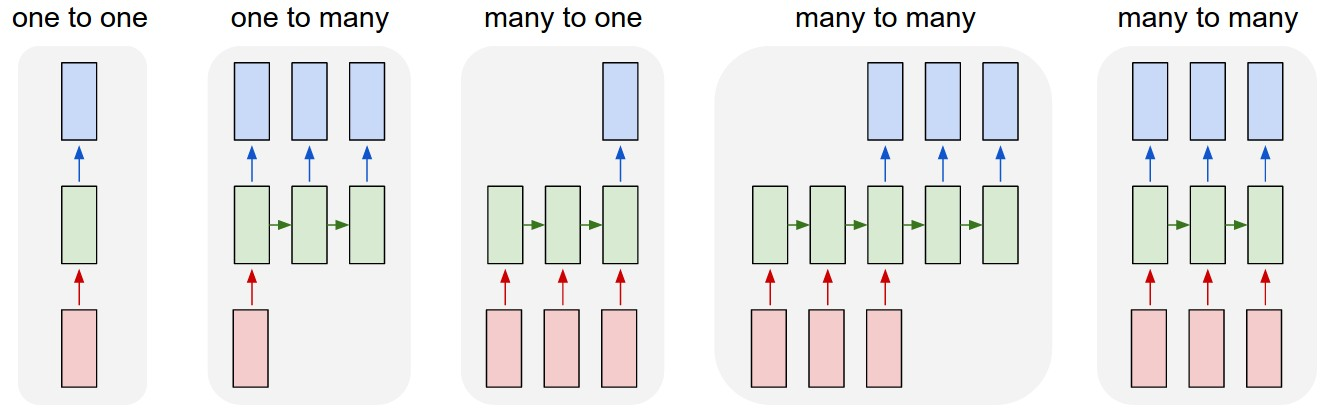
\includegraphics[width=100mm]{diagrams/rnn.jpeg}
	\caption{Rectangles represent vectors, with red being the input, blue the output, and green representing the state of the RNNs. Arrows represent  functions. From left to right: (1) an MLP. (2,3,4,5)  examples of different styles of recurrent neural networks, describing the different types of input and output combinations. (Diagram from \cite{karpathy_unreasonable_2015}). \label{rnn_shapes}} 
\end{figure}

At each time step $t$, a simple RNN produces a hidden vector $h_t$, derived from the input vector $x_t$ and the previous state $h_{t-1}$ in the function $\overrightarrow{h_t} = \overrightarrow{f_w}(h_{t-1}, x_t)$.\footnote{In terms of notation, an arrow over the equations describe the directionality of the model. It is assumed that in the absence of an arrow, sequences go from left to right.}

% talk about arrows and notation properly.
The hidden vector is usually obtained by some affine transformation offset by a bias vector, described in more detail in equation \ref{eq:rnn}. The same function and the same parameters are used at each time step $t$. RNNs, by design, are not computationally parallelisable. This hidden vector $h_t$ is continuously updated as it traverses through the RNN, learning the temporal relationships between the inputs.

\begin{figure}[!ht]
\begin{equation}
\label{eq:rnn}
\begin{aligned}
	h_t &= tanh(W_{hh}h_{t-1}+W_{xh}x_t)
\\
y_t &= W_{hy}h_t
\end{aligned}
\end{equation}
\captionsetup{labelformat=empty}
\caption{Equations for the RNN cell.}
\end{figure}

% talk about how they can be stacked.
RNN cells can be stacked, making a deeper recurrent network, and can also be bi-directional. Bi-directionality explores the temporal relationships of the sequence in both directions (left to right, and vice versa.) This is made possible by stacking two recurrent cells on top of each other, and having one forward propagate in one direction, and another in the opposing direction.

RNNs are typically trained with backpropagation through time (see equation \ref{eq:btt}) The gradient flow $w \leftarrow w - \alpha ({\delta L}/{\delta w})$ is computed at every timestep, meaning that every path from $W$ to the loss $\mathcal{L}$ needs to be considered.

\begin{equation}
\label{eq:btt}
\begin{aligned}
	\frac{\delta L}{\delta w} = \sum^T_{j=0}\sum^j_{k=1}\frac{\delta L_j}{\delta y_j}\frac{\delta y_j}{\delta h_j}(\begingroup\color{brown}\prod^j_{t=k+1}\frac{\delta h_t}{\delta h_{t-1}}\endgroup)\frac{\delta h_k}{\delta w}
\end{aligned}
\end{equation}

Typically, there are two caveats with training RNNs. Firstly, the product (in brown) within the loss function in Equation \ref{eq:btt} causes both vanishing and exploding gradients, either of which make RNNs especially difficult to train. The magnitude of this issue increases as the sequences increase in length. This is compounded by the fact that the limited expressibility of the gradients means that relationships between timesteps earlier in the recurrent computation are harder to learn than timesteps further in the sequence. This is described as the long range dependency problem.

Additionally, it is also difficult for RNNs to establish relationships between potentially relevant non-contiguous inputs and outputs, especially in the case of longer sequences. There is not necessarily a clear indicator in the architecture facilitating this feature, which becomes a problem for translation (e.g. languages with a differing lexical order, such as English and German.)

That being said, RNNs remain appropriate for language modelling primarily for their ability to encapsulate temporally contextual relationships within sequences. The idea of using RNNs for language models can be realised in Section \ref{seq2seq}. This paper revolves around the use of recurrent language models in a generative manner.

\subsection{LSTMs and GRUs} 

LSTMs and GRUs are types of recurrent cells, introduced to circumvent the issue of long range dependency problems, and gradient sensitivities that RNN cells suffered.

% you should update the formulas
\begin{figure}[!ht]
\begin{equation}
  \begin{split}
    i_t &= \sigma(W_i \cdot [h_{t-1},x_t] + b_i) \\
    f_t &= \sigma(W_f \cdot [h_{t-1},x_t] + b_f) \\
		o_t &= \sigma(W_o \cdot [h_{t-1},x_t] + b_o) \\
		g_t &= \sigma(W_g \cdot [h_{t-1},x_t] + b_g) \\
		c_t &= f_t \odot c_{t-1} + i_t \odot g_t \\
		h_t &= o_t \odot tanh(c_t) 
  \end{split}
% \quad\leftrightarrow\quad
	\quad\quad
  \begin{split}
		u_t &= \sigma(W_u \cdot [h_{t-1},x_t] + b_u) \\
		r_t &= \sigma(W_r \cdot [h_{t-1},x_t] + b_r) \\
		c_t &= tanh(Ww_{t-1}+U(r_t \odot h_{t-1})) \\
		h_t &= (1-u_{t})\odot h_{t-1} + u_t \odot c_t
  \end{split}
\end{equation}
\caption{Equations for LSTM cells (left) and GRU cells (right).}
\end{figure}
 
LSTM (Long Short Term Memory; \cite{hochreiter_long_1997}) are a type of recurrent cell that retains information based on the previous inputs through the introduction of gated architectures. These gated architectures regulate the flow of information coming to and from the cell, helping to mitigate the issue of gradient sensitivity and improving long range dependencies. Gates of the cell are parameterised and therefore learnable. LSTM cells can be swapped in place with the RNN cells. It has been shown to have a considerably stronger performance for a variety of tasks compared to RNN cells.

GRUs (Gated Recurrent Units; \cite{cho_properties_2014}) are functionally similar to LSTMs, but uses less parameters. Within the GRU architecture, a feature to retain the previous weights remain, but there exists a direct path to the input from the output, allowing a reduction in training time. \cite{chung_empirical_2014} suggests that GRUs were found to perform at least equivalently to LSTMs but show slight improvements on smaller datasets. As there are objectively less parameters for the GRU, it theoretically converges faster than the LSTM.

\section{Autoencoders}
\label{autoencoders}
% need citation
Autoencoders (\cite{e._rumelhart_learning_1986}) are a specialised form of neural networks where the model attempts to faithfully recreate the inputs at the output - forcing the model to learn the properties of the input data. Autoencoders typically have a layer in the model where its dimension is smaller than the input space, therefore representing a dimensionality reduction in the data (Autoencoders can be considered to be a non-linear representation of PCA). Autoencoders within the domain of NLP are popularised through their use in machine translation, word embeddings, and document clustering. 

Autoencoders are composed of two different components, an encoder network $\alpha$ and a decoder network $\beta$, such that $\alpha : X \rightarrow Z$ and $\beta : Z \rightarrow X$. Note that $Z$ is typically smaller in dimension than $X$, otherwise the model would be learning some form of the identity vector, and would trivially pass through the input. Quantifying the performance of the model is deduced by a reconstruction loss formula. This reconstruction loss compares the output of the decoder against the input of the encoder.

% definitely need a diagram for autoencoders
% what is it good for?

% talk about how hard it is to understand the structure of the latent variable and how this prevents us from sampling.
Although the model learns the distribution of the data, unlike PCA one cannot immediately interpret the principal components of the data. In fact, it is difficult to understand the structure of the latent variable, as is the case for understanding the layers of neural networks in general. Additionally, as there is no sampling mechanism within this model, effectively prohibiting any generative capabilities. 

% talk about how important this is in the context of the task.
\subsection{Variational Autoencoders}
\label{variational_autoencoders}

% talk about how this can be a generative model.

Variational Autoencoders (VAEs, \cite{kingma_auto-encoding_2013}) are an adaptation of regular autoencoders. As opposed to learning a fixed latent vector, VAEs force the encoder to learn parameters of a gaussian distribution - a mean $\mu$ and a covariance $\Sigma$, essentially replacing the encoder from the standard autoencoder with a learned posterior \textit{recognition model}, $q_\phi(z|x)$. This component of the autoencoder parameterises an approximate posterior distribution over $z$, using a neural network conditioned on $x$. This consequently allows us to take advantage of recent advances in variational inference.  During the decoder phase, a sample $z$ is generated from a gaussian using the learned parameters $\mathcal{N}(\mu, \Sigma)$, which is then fed into the decoder network, generating our reconstructed prior  $p_\theta(x|z)$. This sampling mechanism allows VAEs to have generative capabilities. With this, one can entirely avoid the encoder network, and augment the mean and variance vectors to sample outputs from the decoder.

\begin{figure}[!ht]
	\centering
	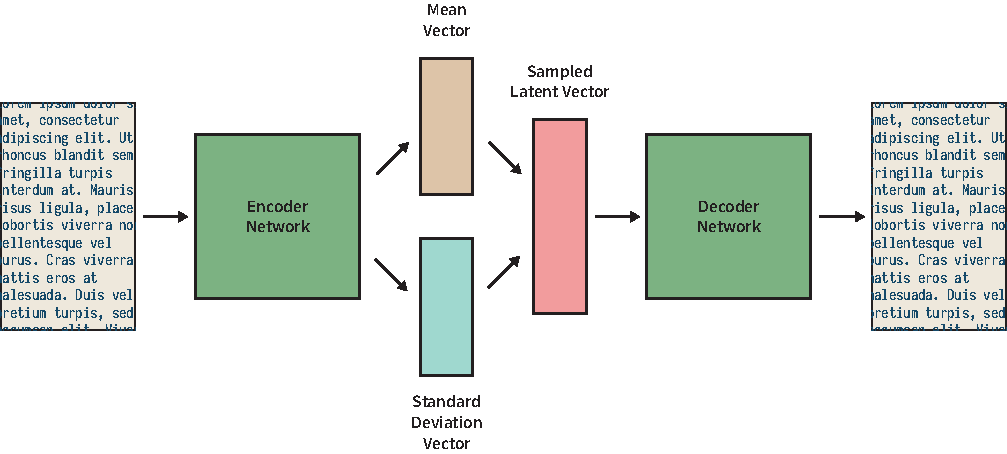
\includegraphics[width=150mm]{diagrams/variational_autoencoders.pdf}
	\caption{An abstracted model architecture for a variational autoencoder, which takes as input some text, and it's predicted output being the same text as the input.\label{vae}}
	\end{figure}
	
For this to be possible, the latent space would learn to represent a non-standard gaussian, which encodes the properties of the inputs.

If VAEs were trained with a standard autoencoder's reconstruction objective, then it would learn to encode its inputs deterministically by making variances in the \textit{recognition model}, $q(\overrightarrow{z}|x)$ vanishingly small (\cite{raiko_techniques_2014}), such that when measuring the influence of the gaussian parameters against a standard gaussian, the difference would be obsolete. This is known as a vanishing KL\footnote{KL stands for Kullback-Leibler, the authors behind the KL Divergence (Equation \ref{eqn:kl_divergence}.)} (\cite{fu*_cyclical_2019}). 

\begin{equation}
	\label{eqn:kl_divergence}
D_{KL}(P ||Q) = \sum_{x \subset X} P(x) \cdot log (\frac{P(x)}{Q(x)})
\end{equation}

Instead, the loss function for VAEs is composed of two components; a reconstruction loss that involves an expectation of the output; and a KL Divergence (see Equation \ref{eqn:kl_divergence}), which helps encourage the learned posterior $q_\phi(z|x)$ to be similar to the true posterior distribution $p(z|x)$. The goal of this loss function would be to find the variational parameters that minimise the divergence, but This would typically be mathematically intractable, as $p(x)$ appears in the evidence. However, the equations can be rewritten, separating the intractable components from the tractable.

\begin{equation}
	\label{eqn:elbo}
	\mathcal{L}(\theta, \phi, x, z) = \mathbb{E}_{q \phi (z|x)}[log \thinspace p_{\theta}(x|z)] - D_{KL}(q_{\phi}(z|x)\thinspace||\thinspace p(z)) \leq log (p(x))
\end{equation}

KL divergence is always greater than or equal to zero, by definition of Jensen's inequality. This means that minimising the KL Divergence is equivalent to maximising the ELBO (Evidence Lower Bound). This loss mechanism (Equation \ref{eqn:elbo})  us to approximate the posterior inference. This objective provides a tractable lower bound on the true likelihood of the data, and forces the model to encode some information on the data into the gaussian parameters.

Note that the ELBO is not necessarily a loss function. To observe how well the model has learned to model properties into the gaussian, we observe the KL divergence. Typically, the larger the better.

% In other words, it is the expectation of the logarithmic difference between the probabilities $P$ and $Q$, where the expectation of $P$ is already known.

\subsubsection*{Reparameterisation Trick}
\label{reparam_trick}

\begin{equation}
	\label{eqn:reparam}
	z = \mathcal{N}(\mu, \Sigma) \equiv \mu + \Sigma \cdot \epsilon
\end{equation}

If $z$ was generated in exactly the method described above, calculating gradients through backpropagation would be impossible as gradients would have to eventually push through a randomly sampled latent variable. The gaussian reparameterisation trick (\cite{kingma_auto-encoding_2013}) subverts this issue through the rearrangement of the gaussian parameters. Instead of sampling $z$ through a gaussian $\mathcal{N}(\mu, \Sigma)$, $z$ can be redefined with a summation of $\mu$ and some gaussian noise $\epsilon \sim \mathcal{N}(0,1)$ applied to $\Sigma$ (See Equation \ref{eqn:reparam}). This rearrangement allows for derivatives to be calculated with respect to the parameters that are needed for learning as derivatives with respect to the relevant components would cancel out $\epsilon$ (thus making learning possible).

\subsection{Conditional Variational Autoencoders}
\label{conditional_variational_autoencoders}
In a VAE, the decoder cannot typically produce outputs of a particular condition on demand - the description for the VAE matches the definition of semi-supervised learning. CVAEs add to the VAE to include conditioning on another description of the data, a conditioning descriptor $y$. 

\begin{figure}[!ht]
	\centering
	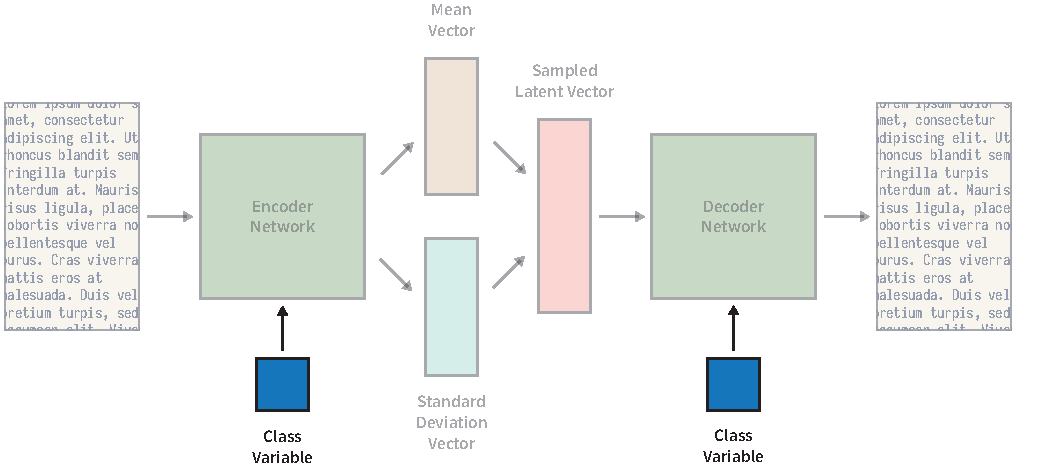
\includegraphics[width=150mm]{diagrams/conditional_variational_autoencoders.pdf}
	\caption{A model architecture for a CVAE, which includes the label being fed into the encoder and decoder networks. \label{cvae_diagram}}
\end{figure}

During training time, a condition (represented by some arbitrary vector) is fed at the same time to the encoder and decoder. After training, to generate an output that depends on $y$ we feed that datum to the decoder along with a random point in the latent space sampled from a standard normal distribution.

Samples can be generated from the conditional distribution $p(x|y)$. By changing the value of $y$, we can get corresponding samples $x \sim p(x|y)$. The system no longer relies on the latent space to encode what output is necessary; instead the latent space encodes other information that can distinguish itself based on the differing $y$ values.

In terms of implementation, it happens to be more feasible to concatenate the conditioning variable to the input prior to feeding them into the encoder. In the event of inference (where samples are generated independently of the encoder), one can concatenate $y$ with some arbitrary conditional vector $z$ into the decoder to generate outputs. This keeps the model from needing to adjust its architectural characteristics in order to accomadate the conditioning variables.

\section{Related Work}

% why?

\subsection{Sequence To Sequence}
\label{seq2seq}

Sequence to Sequence, (Seq2Seq, \cite{sutskever_sequence_2014}) is a type of neural network model that models relationships between sequences.  Seq2Seq comprises of two components, encoders and decoders (in a similar fashion to autoencoders), both of which are represented with RNN models (although as explained earlier, can be replaced with LSTM or GRU cells). Defining Seq2Seq as a language model, it takes a pair of sequential data, which within the contexts of text generation, would be query and response sequences. The model would take in the query sequence, and attempt to recreate the response. The query sequence would go through the encoder model. The last hidden state value of the encoder is used as the context variable, which encodes the characteristics of the input sequence. This is used as the first hidden vector value for the decoder, which would then predict the response sequence. This sequence can be visualised in Figure \ref{seq2seq_diagram}. For the purposes of this paper, we describe this as the standard recurrent language model.

\begin{figure}[!ht]
		
\centering
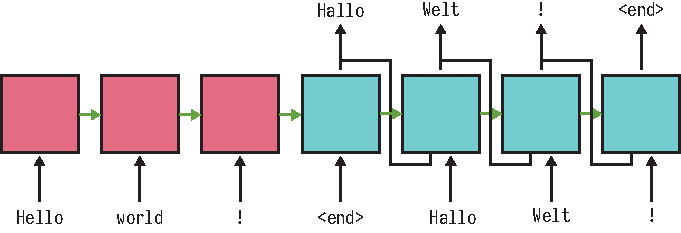
\includegraphics[width=100mm]{diagrams/seq2seq.pdf}
\caption{An abstracted model of the Seq2Seq architecture, where the encoder (pink) takes in the input sequence, and the decoder (blue) shows the output sequence. The encoder outputs are effectively ignored. \label{seq2seq_diagram}}
\end{figure}

Seq2Seq models have shown to be effective in response generation, but is not without its own set of problems. For instance, the context variable itself is considered to be the bottleneck as it has to encompass the properties of the entire input sequence in a single vector. As Seq2Seq is based on RNNs, they are also subject to vanishing and exploding gradients (Section \ref{rnn}), and that it becomes increasingly difficult to retain information about earlier parts of the sequence as opposed to recent parts of the sequence in the encoder stages as a consequence. A popular approach to improving long term dependencies exists however, with the introduction of attention mechanisms, discussed in Section \ref{seq2seq_attn}.

Furthermore, the responses produced from a Seq2Seq model naturally lacks lexical diversity and richness (\cite{serban_hierarchical_2016}, \cite{zhao_learning_2017}, \cite{jiang_why_2018}). There tends to be many causes, but one reason (which we explore in the paper) is due to the lack of statistical inferencing. The model itself lacks the possibilty of presenting a variety of lexical responses in the decoder, in a manner that a VAE could through the sampling of a latent vector.

\subsubsection{Attention Mechanism}

\begin{figure}[!ht]
      
	\centering
	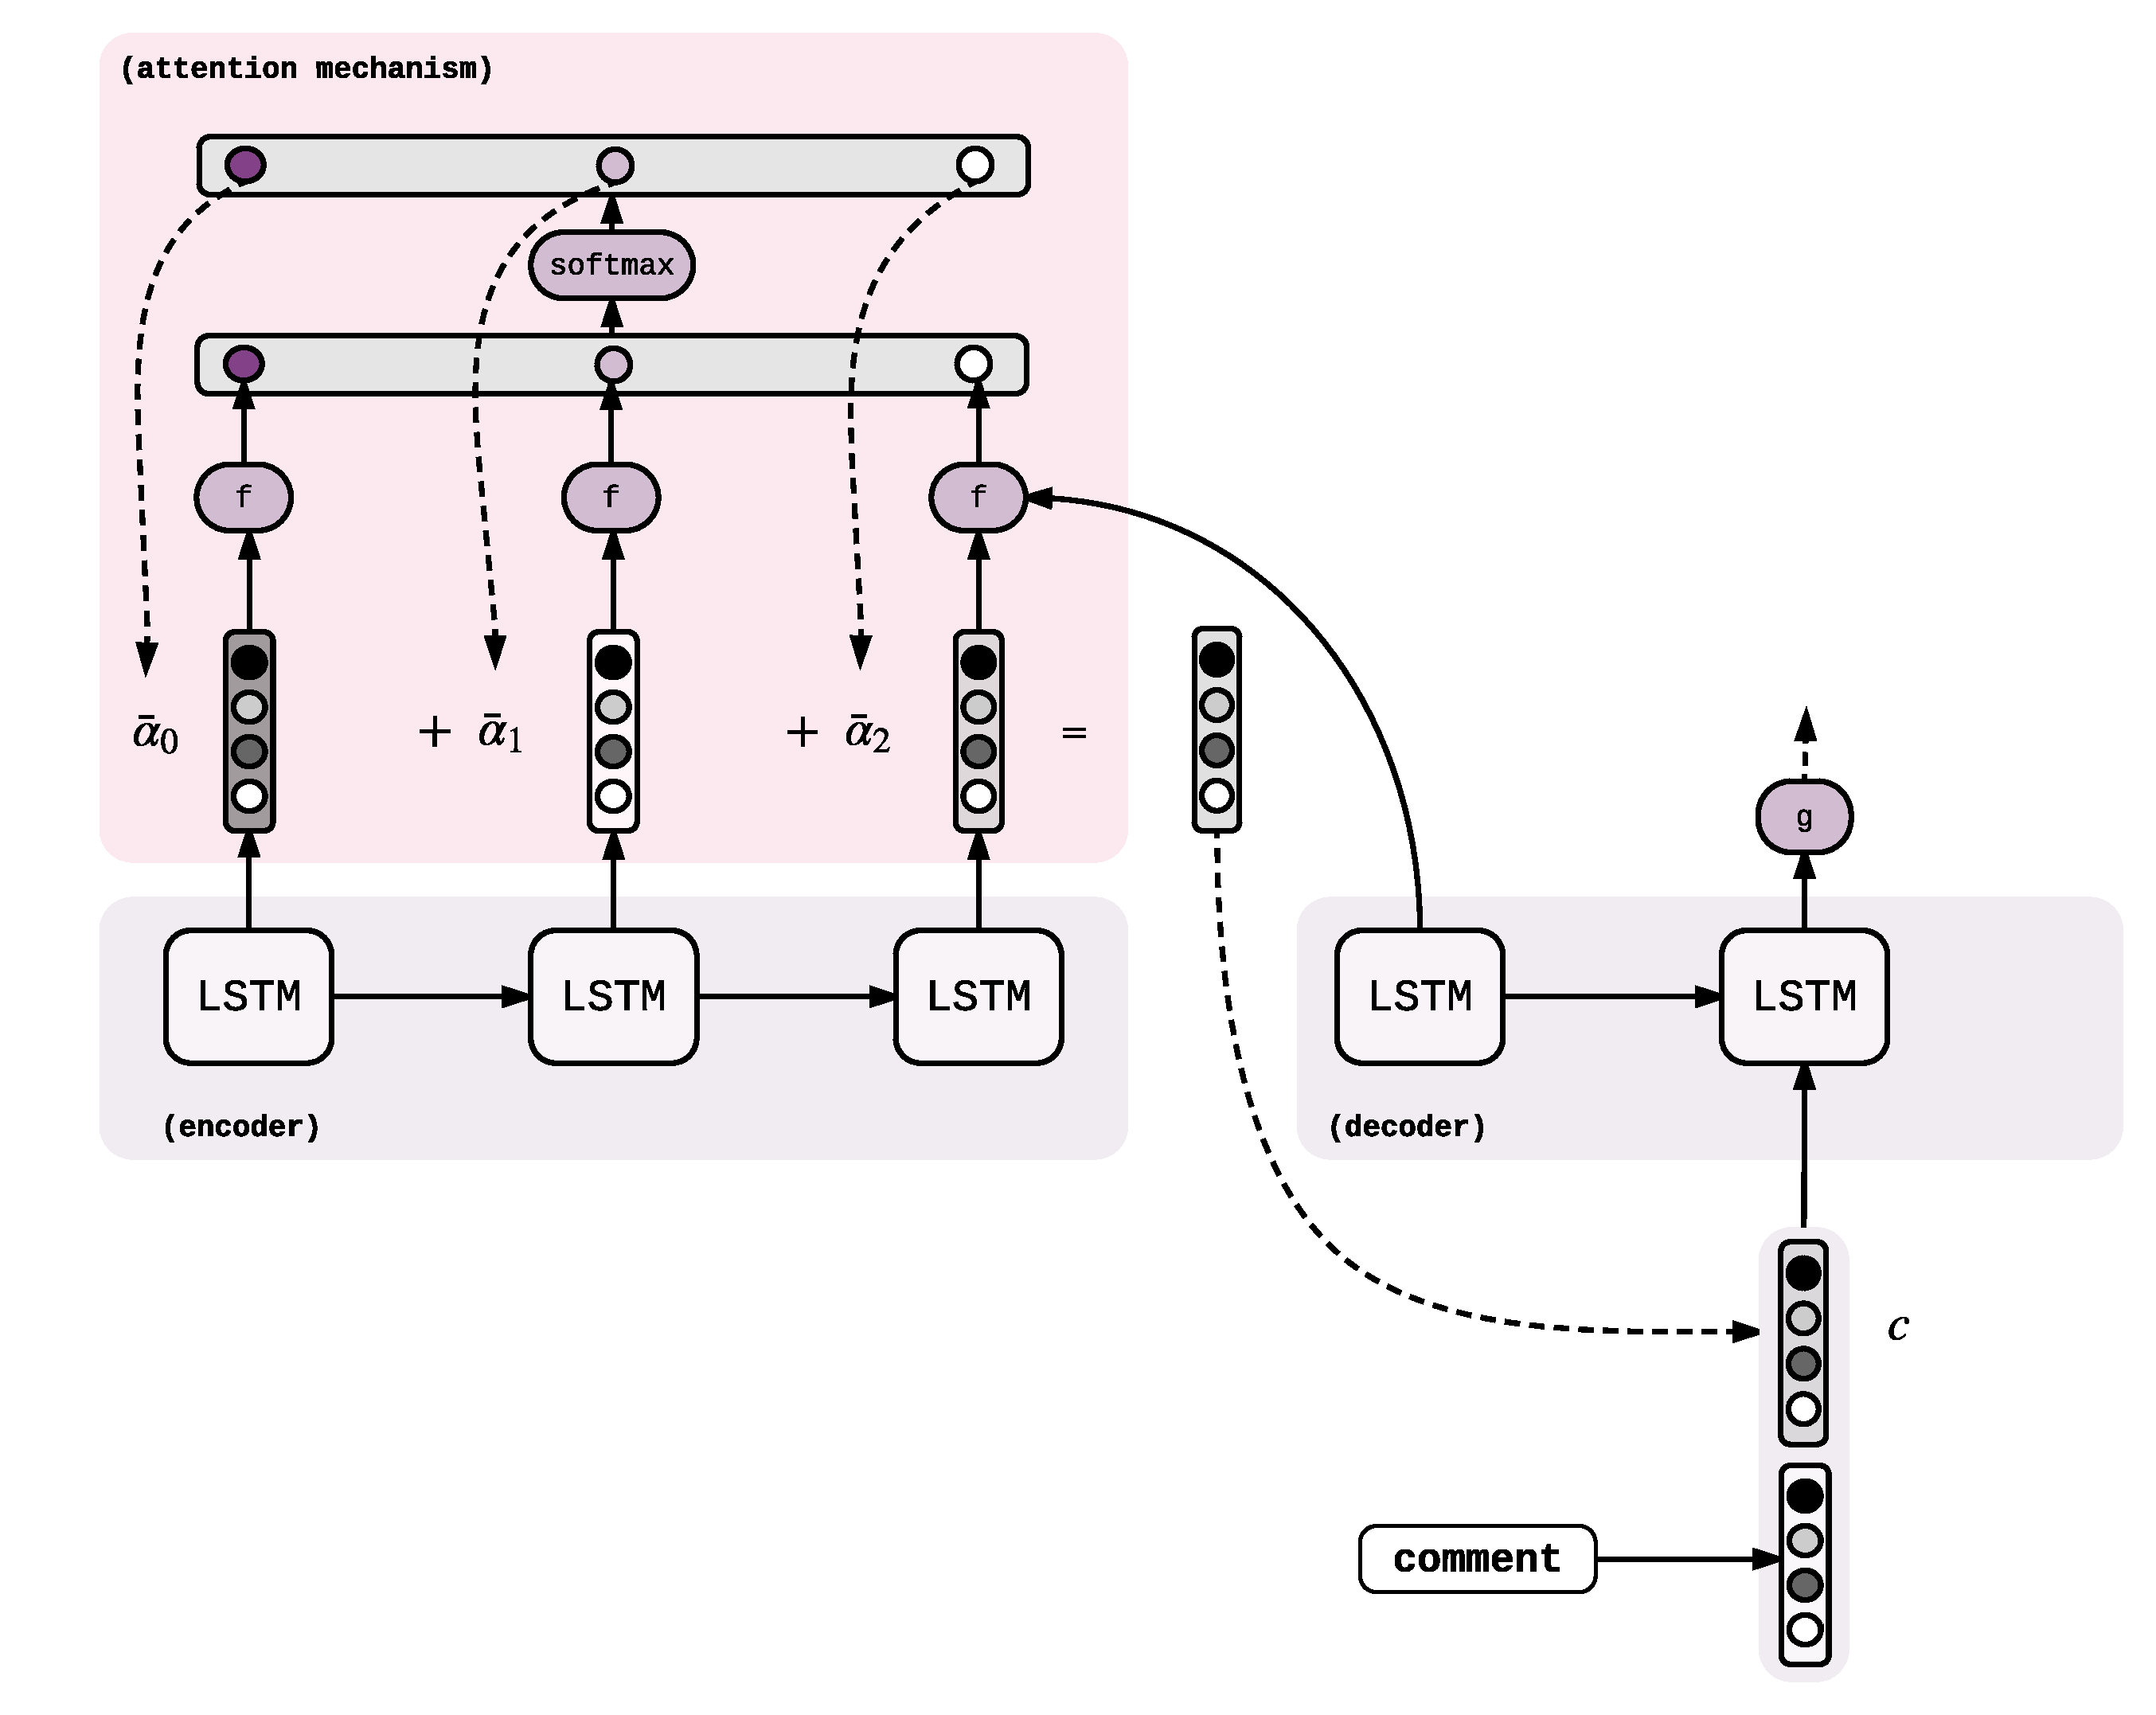
\includegraphics[width=100mm]{diagrams/seq2seq_attention_mechanism.pdf}
	\caption{An abstracted diagram of the attention mechanism, applied to a Seq2Seq model. (Diagram from \cite{genthial_seq2seq_2017})\label{seq2seq_attn}}
\end{figure}

% need to elaborate on this.

In addition to the context vector, the decoder can also retrieve non-contiguous relationships on the encoder values using attention (\cite{bahdanau_neural_2014}). This mechanism, when applied to Seq2Seq,  looks at all of the hidden states from the encoder outputs, and generates  relationships between these outputs against the decoder output. This allows the decoder network to ``attend'' to different parts of the source at each step of the output generation, learning relevant non-contiguous relationships between the query and response sequences. Attention mechanisms would work in tandem with the context vector provided from the encoder, helping the model with long-range dependency problems.

Attention mechanisms were found to perform particularly well in machine translation problems where languages which are arbitrarily aligned, and has eventually led to the creation of transformer models (\cite{vaswani_attention_2017}), avoiding the use of recurrent networks altogether.

\subsection{Variational Sequence To Sequence}
\label{variational_context}

Instead of passing through the last hidden state from the encoder to the decoder, it is possible to encode the context variable produced from the encoder in the form of gaussian parameters in a similar fashion to VAEs. This is known as a variational sequence to sequence network (\cite{bowman_generating_2015}), but for the remainder of this paper we refer to them as Bowman models. The intention of this model is to learn the high level global syntactic features of the input data into the latent vector. This is such that when inference occurs, the model could generate unconditioned sequences which looks like the input data. This is typically described as representation learning.

The encoder RNN takes the input sequence, and produces a hidden vector. This is used to encode the parameters of the gaussian, which define the latent vector. During the decoder phase, a sample latent vector is produced (in a similar manner to VAEs), which is then fed as the hidden vector for the decoder RNN, which also takes the input variables and attempts to recreate the input in an autoencoder fashion.

% representation learning

\begin{figure}[!ht]
	\centering
	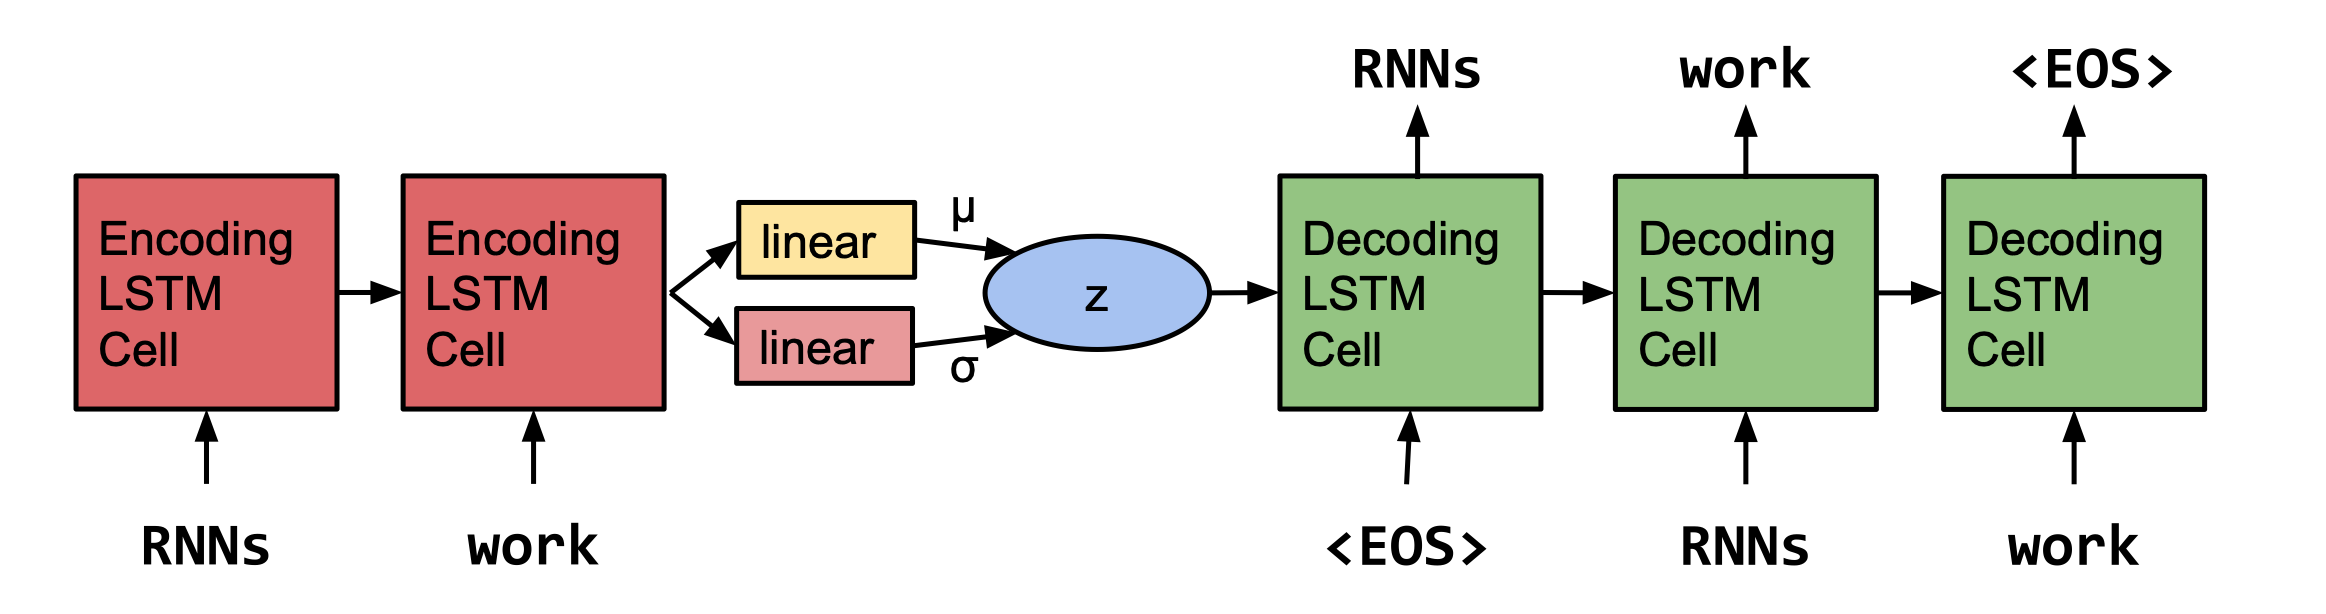
\includegraphics[width=100mm]{diagrams/seq2seqvae.png}
	\caption{The core structure of the VAE language model - words are represented as embedded vectors (Diagram from \cite{bowman_generating_2015}). \label{vae_seq2seq}}
\end{figure}

The model is trained in a similar fashion to VAEs where the overall loss is composed of a reconstruction loss and a KL divergence (see Equation \ref{eqn:elbo}). However, it also utilises additional mechanisms to force the language model to encode features into the gaussian parameters. We explain these features in further detail in Section \ref{optimisation_challenges}.

As described above, it is not necessarily designed for conditioned discourse generation. Even if it were modified for that specific purpose, the responses would be generated from the same latent variable, restricting its variability in responses. (\cite{zhao_learning_2017}; \cite{du_variational_2018}) With that being said, it remains important for discussion as it handles optimisation challenges in a manner which we could leverage later on for our model of choice.

\subsection{Conditional Variational Sequence to Sequence}

\begin{figure}[!ht]
	\centering
	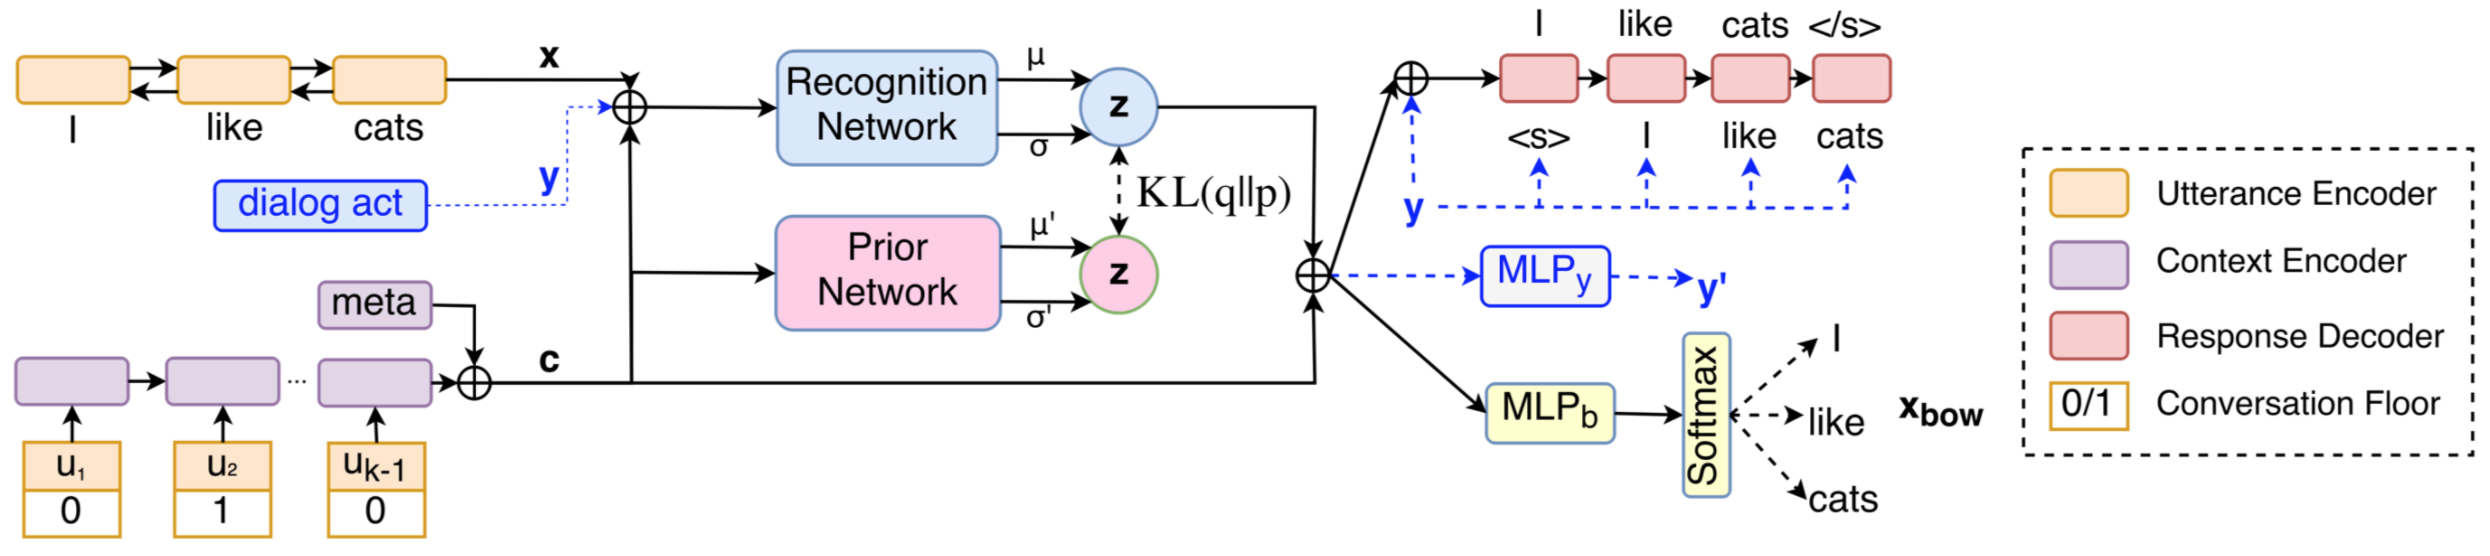
\includegraphics[width=120mm]{diagrams/cvae_seq2seq.png}
	\caption{The structure of the CVAE language model. (Diagram from \cite{zhao_learning_2017}). \label{cvae_seq2seq}}
\end{figure}

Conditional Variational Sequence to Sequence (CVAE Seq2Seq; \cite{zhao_learning_2017}) is an extension of Bowman's model for the purposes of discourse generation. It includes a plethora of additional components, including attention mechanisms to make discourse generation more viable. The model takes as input some query sequence as the condition, and attempts to generate a response sequence.

Leveraging Bayesian inference, the CVAE defines the conditional distribution $p(x,z|c) = p(x|z,c)\cdot p(z|c)$, where $z$ represents a gaussian latent variable, and $c$ corresponds to the context vector, produced from the attention mechanism. The model's goal was to leverage neural networks (parameterised by $\theta$) to approximate $p(x|z,c)$, which in a bayesian setting is described as the likelihood and $p(z|c)$ being the prior. 

In a Bayesian setting, the prior represents beliefs on some quantity before some additional information (in the form of evidence) is taken into account. CVAE uses prior knowledge in the greedy decoder to help generate diversity in responses. The generative process for $x$, seen in Figure \ref{cvae_seq2seq} is as follows:

\begin{itemize}
	\item Sample a latent variable $z$ from the prior network $p_\theta (z|c)$.
	\item Generate $x$ through the response deocder $p_\theta(x|z,c)$.
\end{itemize}

The model is trained to maximise the conditional likelihood of $x$, given $c$. This involves the intractable marginalisation over $z$, but this has been discussed to be trainable using the ELBO loss with Formula \ref{eqn:elbo}. 

Once a latent variable is generated (notice that it is the case that the latent $z$ is generated once during the decoder phase), it is fed to the decoder model to predict words in $x$ sequentially. This diverges from Bowman's model, where the words are pushed in one go. 

One of the paper's novel contribution is an auxiliary function described as a bag of words loss. Within the NLP domain, a bag of word refers to a set of unique words. The model's loss function revolves around using the latent variable $z$ within its model to predict the set of output words (in no particular order) as a multi-class one-hot value. The model we discuss in the next chapter will go into the bag of words loss in more detail.


\chapter{Model}

% mention the limitations of Seq2seq for your problem and ways they could be addressed (VAEs, etc.), describe the VAE approach and your motivation to pick it, introduce the VAE paper you work with in details.

In this chapter we focus on an approach called the Variational Autoregressive Decoder (VAD). The model itself is a combination of the components and models described in the literature review (Chapter \ref{lit_survey}). To better understand the capabilities of the VAD, we subject it to a series of datasets to understand how it works and its performance against them. The VAD has been shown to better encapsulate a distribution of the data within the latent parameters than the CVAE Seq2Seq, and retains a higher KL ratio respective to its overall loss function. This model is used as the candidate mechanism for encapsulating the dataset (for our problem domain), which could be sent to clients.

\section{Variational Autoregressive Decoders}

Variational Autoregressive Decoders (VADs; \cite{du_variational_2018}) extends CVAE Seq2Seq by introducing multiple latent variables into the autoregressive Decoder at different time-steps. This allows the decoder to produce a multimodal distribution of text sequences, allowing a greater variety of responses to be produced than what is possible with the CVAE Seq2Seq.

\begin{figure}[!ht]
		
	\centering
	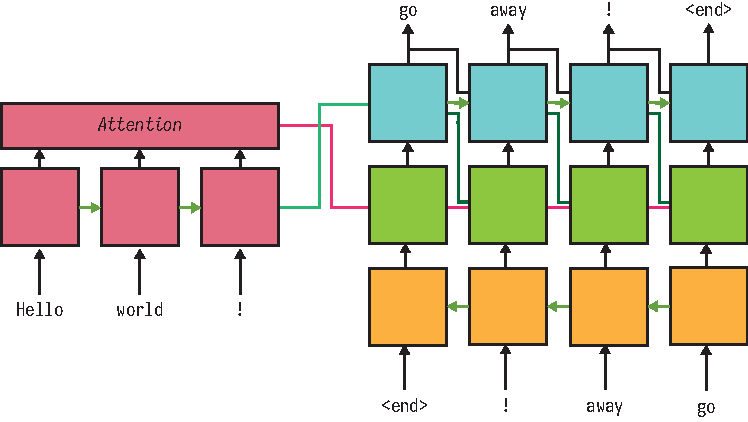
\includegraphics[width=100mm]{diagrams/vad.pdf}
	\caption{An abstracted diagram of the VAD model, where the encoder (pink) takes in the input sequence, orange represents the backwards model, green represents the latent context generation, and the decoder (blue) shows the output sequence.\label{vad_abstract}}
	\end{figure}

VADs use the vanilla Seq2Seq architecture as the base (Section \ref{seq2seq}) taking as input, sequences $x = \{x_1, x_2, ..., x_n\}$, and $y = \{y_1, y_2, ..., y_m\}$ representing the query and response sequences respectively. Both the encoder and decoder use GRUs, with the encoder utilising a bidirectional GRU, and the decoder being unidirectional. For each timestep $t$, each GRU in the decoder network is encoded with hidden state $h^d_t$. The components of the model are broken down into their subsections below.

\subsection{Architecture}
% need a diagram

\subsubsection{Encoder}

\begin{align}
\label{eqn:eqlabel}
\begin{split}
	\overrightarrow{h^e_t} = \overrightarrow{GRU}(x_t, \overrightarrow{h^e_{t-1}})
\\
\overleftarrow{h^e_t} = \overleftarrow{GRU}(x_t, \overleftarrow{h^e_{t+1}})
\end{split}
\end{align}

The encoder works in a similar fashion to the encoder described in the Seq2Seq network. The only difference being that the encoder described in the implementation leverages bi-directionality. Similarly to the Seq2Seq and other recurrent language models, the last hidden vector is passed through as the initial hidden vector for the decoder model.

\subsubsection{Backwards and Attention}


% you should update the formulas
\begin{figure}[!ht]
	\label{eqn:eqback}
	\begin{equation}
		\begin{split}
			\overleftarrow{h^d_t} &= \overleftarrow{GRU}(y_{t+1}, \overleftarrow{h^d_{t+1}})
		\end{split}
	% \quad\leftrightarrow\quad
		\quad\quad
		\begin{split}
			\alpha_{s,t} &= f_{attention}([h^e_d, h^d_{t-1}]) \\
			c_t &= \sum^m_{s=1}\alpha_{s,t} h^e_s
		\end{split}
	\end{equation}
	\caption{Equations for Backwards (left) and Attention (right).}
	\end{figure}


The backwards RNN (only activated during training) is used to feed additional contextual information to the inference model.  During training, the backwards RNN takes as input the training outputs $y$ and outputs hidden vectors in a reverse, sequential manner. The VAD leverages the attention mechanism in a similar fashion to Seq2Seq; it  takes in the input sequence, and is contextualised by the decoder's previous hidden output at each time step.

\subsubsection{Decoder}
\begin{figure}[!ht]
	\centering
	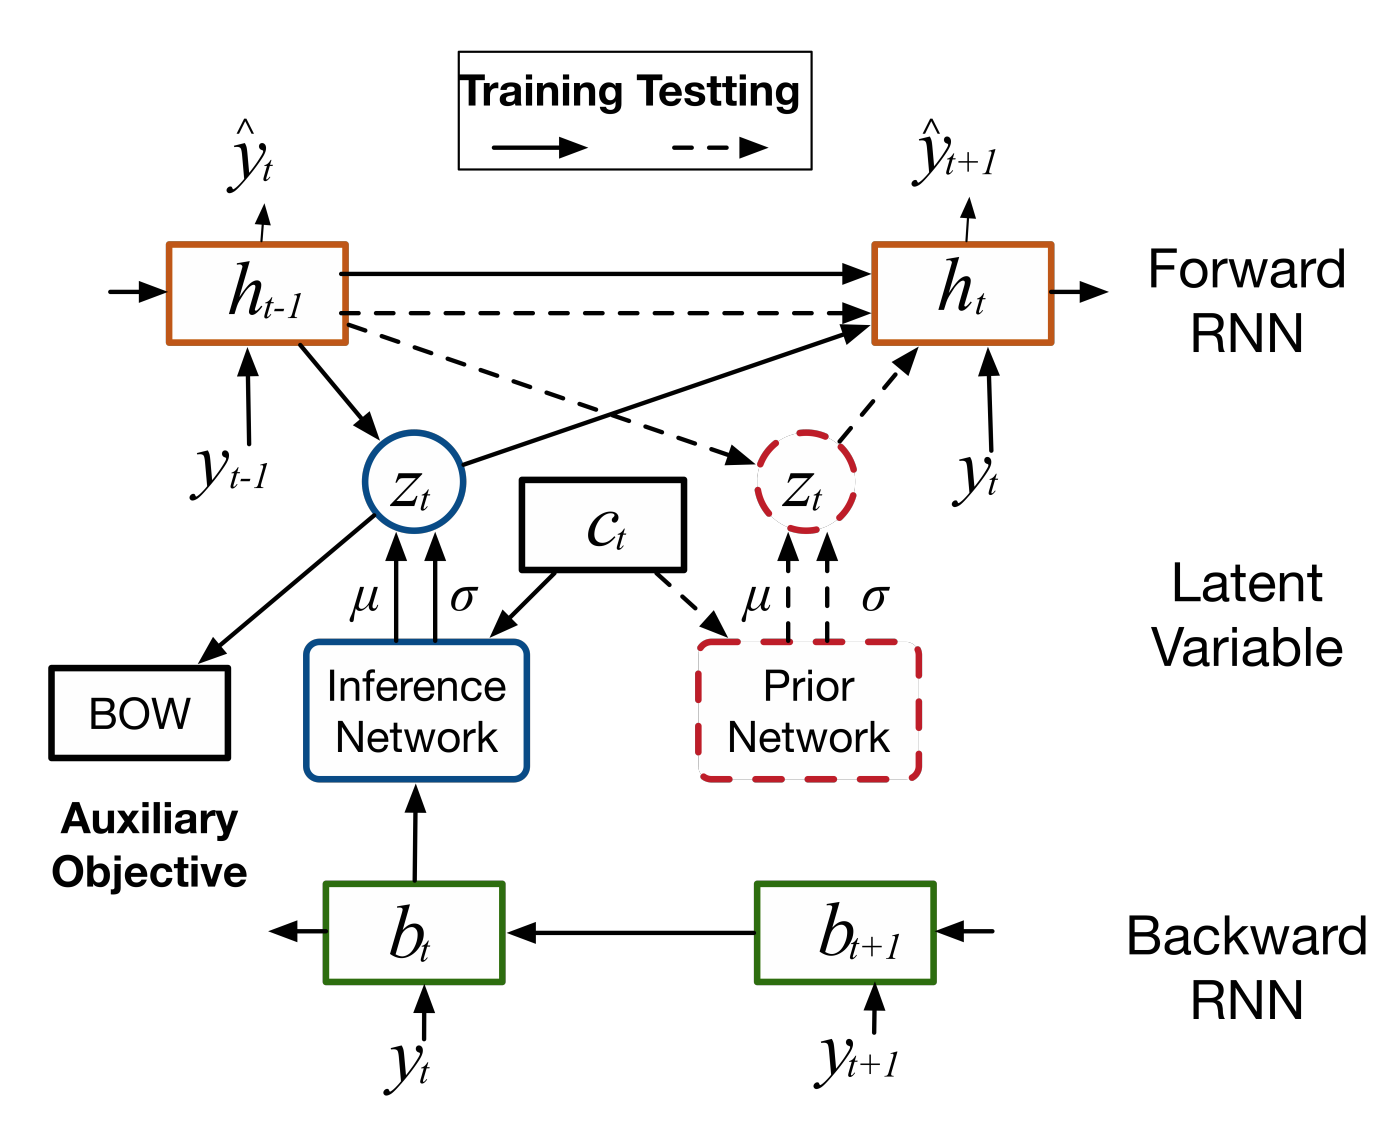
\includegraphics[width=80mm]{diagrams/vad_decoder.png}
	\caption{A High level diagram of the decoding component of the VAD. (Diagram from \cite{du_variational_2018})\label{r:vad_decoder}}
	\end{figure}
	
The decoder component of the model comprises multiple sub-components, each of which are described in detail below. The sampling mechanism is within this decoder, which differs from other variational approaches - Earlier approaches sample a latent variable outside the decoder phase.

\subsubsection{Inference and Prior Models}

\begin{figure}[!ht]
	\label{eqn:inf_prior}
	\begin{equation}
		\begin{split}
			\lbrack \mu^i, \sigma^i \rbrack &=
			f_{infer}([\overrightarrow{h^d_{t-1}}, c_t, \overleftarrow{h^d_t}])
			\\
			q_{\theta}(z_t|\boldsymbol{y}, \boldsymbol{x}) &= \mathcal{N}(\mu^i, \sigma^i)
		\end{split}
	% \quad\leftrightarrow\quad
		\quad\quad
		\begin{split}
			\lbrack \mu^p, \sigma^p \rbrack &=
			f_{prior}([\overrightarrow{h^d_{t-1}}, c_t])
			\\
			p_{\phi}(z_t|\boldsymbol{y}_{<t}, \boldsymbol{x}) &= \mathcal{N}(\mu^p, \sigma^p)
		\end{split}
	\end{equation}
	\caption{Equations for Inference (left) and Prior (right) models.}
	\label{inf_prior}
	\end{figure}

The inference model attempts to learn a conditional posterior distribution $z_t$ using the backward output at that timestep $\overleftarrow{h^d_{t-1}}$, the attention context $c_t$, and the decoder outputs $\overrightarrow{h_{t-1}}$. $z_t$ is created using the gaussian reparameterisation trick described in Section \ref{reparam_trick}.

This component stems away from \cite{zhao_learning_2017}, as $\boldsymbol{z}$ is now decomposed into sequential variables $\boldsymbol{z} = \{z_1,...,z_t\}$, which are generated at each time step of the decoder phase.  \cite{du_variational_2018} suggests that this conditioning allows the latent variables to be guided for long-term generation.

The prior network is restricted to using observable variables during testing of the model to generate $z_t$ using only observable information $c_t$ and $h^d_{t-1}$; i.e. the inference model is not used to generate $z_t$ during testing. It is designed in a similar fashion to the decoder network where the input variables are concatenated together, which can be seen in Equation \ref{inf_prior}. 

\subsubsection{Forward RNN}


\begin{equation}
	\begin{split}
		\overrightarrow{h^d_t} &= \overrightarrow{GRU}([y_{t-1},c_t,z_t], \overrightarrow{h^d_{t-1}}) \\
		p_\phi(y|\boldsymbol{y}_{<t},\boldsymbol{z}_t, \boldsymbol{x}) &= f_{output}([\overrightarrow{h^d_t}, c_t])
	\end{split}
\end{equation}

The decoder then takes in $z_t$, alongside the previous output $y_{t-1}$ and the context vector produced from the attention mechanism $c_t$ to produce the response $y_t$.

\subsection{Auxiliary Objective}
\label{aux_obj}
One of the novel contributions of the model is the use of a temporally contextual auxiliary objective that uses the sampled latent vector $z_t$ to predict the sequential bag of words (SBOW) of the response sequences $\boldsymbol{y}_{bow}(t+1,T)$. Let $f=MLP_b(z_t) \in \mathcal{R}^V$ where $V$ be the vocabulary size, then the bag of words can be deduced using the following equation:

\begin{equation}
	log [p_\xi(y_{bow(t+1,T)}|z_{t:T}) ] = log  \frac{e^{f_{z_{t}}}}{\sum^V_j e^{f_{j}}}
\end{equation}

The intuition is that this auxiliary objective helps to improve the KL divergence, as the latent variables would capture the information from a different perspective (\cite{du_variational_2018}).

\subsection{Learning Mechanism}


VADs uses the ELBO (Equation \ref{eqn:elbo})\footnote{As the KL divergence no longer compares the latent variable against a standard gaussian, we derive the equation to allow gradient propagation between two arbitrary distribution. This can be seen in the Appendix (Section \ref{kl_derivation}).} and a weighted negative log likelihood loss of the auxillary objective, controlled by $\alpha$. This loss is computed at each timestep, and is then summed at the end of the sequence generation during the decoder stage. During training and evaluation, we sample both the inference and prior models to facilitate measuring the loss.
% The KL divergence allows the model to perform discourse generation using the prior model, by forcing it to decode plausible sentences from every point in the latent space that has some reasonable odds under the prior (\cite{bowman_generating_2015}).

\begin{equation}
	\begin{split}
		\mathcal{L} &= \sum_t [\mathcal{L}_{ELBO}(t) + \alpha \mathcal{L}_{AUX}(t)] \\
		\mathcal{L} &= \sum_t [(\mathcal{L}_{LL}(t) - \mathcal{L}_{KL}(t)) + \alpha \mathcal{L}_{AUX}(t)] 
	\end{split}
\end{equation}

During implementation, it was found that the auxiliary loss weight $\alpha$ typically initially increases the KL divergence, but eventually produces a diminishing effect to both the auxiliary loss and the KL divergence. Attempts to contact the original authors of the VAD paper were to no avail, and is left for future work. Presently, we set $\alpha=1$. 
 
% Although these models have been used in NMT related problems, sequence generation is often unexplored within NLP. We propose using models that traditionally perform well in NMT problems and adapt them for use with sequence generation problems. 

\section{Optimisation Challenges}
\label{optimisation_challenges}

In addition to the fact that recurrent networks themselves are difficult to train (see Section \ref{rnn}), it may occasionally be the case that with variational models, the sampled latent variable $z$ is often ignored during training. Ideally, a model that encodes useful information in $z$ will have a non-zero KL divergence term in addition to a relatively small negative log likelihood loss. 

Due to the sensitivity of the latent component, early implementations of the VAD would often ignore $z$ and go after the low hanging fruit during the learning process of the decoder. $z$ would encorporate a lack of relevant information and is essentially ignored. That is not to say that the model does not learn - it would rather allocate more learning weight to the information from other inputs such as the attention mechanism and the encoder's hidden value.

The absence of learning in $z$ results in a KL collapse (or Vanishing KL), such that the KL loss reaches zero, indicating that the posterior distribution of $z$ has ``collapsed'' under the prior. This effectively renders $z$ to be ignored, and thus the model is then effectively equivalent to an RNN language model. (\cite{bowman_generating_2015}) Although we explain one of the mechanisms used to prevent KL collapse with the auxiliary objective (see Section \ref{aux_obj}), we will also discuss some additional approaches to overcome learning difficulties, primarily around $z$, but also for the model overall.

\subsection{KL Annealing}

KL Annealing is a simple approach by \cite{bowman_generating_2015}, it involves adding a variable weight to the KL term in the cost function during training. Initially, the weight is zero, forcing the model to encode as much information into the latent variable as it can. The weight is then gradually increased, eventually reaching 1. At this stage the weighted cost function is equivalent to the ELBO loss. This could be thought of as annealing from a regular autoencoder towards a variational one.

That being said, Bowman et al. exposes a variety of additional hyperparameters including the step size, the total number of steps, the step rate (for instance, a linear progression or a logistic). For the sake of simplicity, we explore a linear approach with a fixed linear progression.

\subsection{Word Dropout}
Also proposed by \cite{bowman_generating_2015}, Word Dropout involves weakening the decoder by removing some conditioning information during training. This is done by randomly replacing a fraction of the conditioned-on word tokens with a generic unknown token UNK, which forces the model to depend on the latent variable $z$ for prediction. This works in a similar fashion to the standard dropout (\cite{srivastava_dropout:_2014}) where connections are dropped between layers of a network, but is instead applied to the input data of a recurrent cell. We do not explore this technique further for the VAD as a case by \cite{bowman_generating_2015} suggests that it could disrupt the performance of the model when the drop rate is sufficiently high.

\chapter{Experimental Setup}

To explore the performance of the VAD, we benchmark its performance against two other models: a baseline model, and the Bowman model (see Section \ref{variational_context}). The Seq2Seq model and the Bowman models were chosen for comparison not necessarily to compare state-of-the-art performance but to verify the correctness of the implementations of our VAD model. We do not implement the CVAE Seq2Seq model as it is not the focus of this ISO.

The baseline model represents a vanilla encoder-decoder Seq2Seq network (\cite{sutskever_sequence_2014}; Section \ref{seq2seq}) that uses the same architectural base as the VAD but only minimises the standard negative log likelihood loss (i.e. the KL divergence computations are not computed). We use this approach since KL collapse on variational models is effectively equivalent to a recurrent language model.

As stated earlier, the Bowman model is primarily designed for language modelling, whereas the VAD is designed for response generation. With this prior knowledge it was expected that the Bowman model would perform worse than the VAD model for all tasks, but it remains important to understand from a variational standpoint, what a KL baseline should be.

% With the VAE seq2seq model, it is not necessarily designed with the intention of neural response generation, and that it was expected that the VAE seq2seq model would perform poorly in our scenario. However, to standardise the measurements for results, we pad the sequences such that it would still be useful for measuring the expected KL and reconstruction losses for a simple recurrent language model.

\subsection*{Weight Initialisation}

Typically, we intend to have the weights asymmetricly generated; i.e. have random starting positions for gradient descent, which would enable us to have a better chance of finding the minimum as opposed to having starting points that would somewhat correlate with each other.

\cite{glorot_understanding_2010} proposed to initialise the weights based on a gaussian $Var(w)=\mathcal{N}(0,\frac{2}{|n_{in}| + |n_{out}| })$ where $w$ represents a layer in a network, and $|n_{in}|$ represents the number of neurons feeding into it, and similarly so for $|n_{out}|$. Note this description uses a gaussian distribution, but this could also be uniform. This method has shown a lot of success for sigmoidal and tanh based activation functions. We initialise the weights for all models with this approach.

\subsection*{Teacher Forcing}

Teacher Forcing (\cite{williams_learning_1989}) is a concept of using real target outputs for the next input in the decoder sequence of RNNs as opposed to using the decoder's prediction. This causes the model to converge faster, but may exhibit instability when the trained network is exploited. Typically, this can be controlled with a probability $p$ such that the decoder sequence has a $p$ chance of using teacher forcing during training.

With teacher forced decoders, outputs that read with coherent grammar can be observed, but the generated responses can wander far from the correct response; i.e. with some $p<1$, some outputs from the decoder at some timestep would be correct, but the others would have a chance to completely change the semantics of the output. As the purposes of this paper is to explore artificial texts, we set the VAD and Seq2Seq teaching probabilities $p=1$, but not the Bowman model as it is not applicable\footnote{As stated earlier, the responses are generated in its entirety in one operation, and not necessarily separated with  recurrent steps.}.

\subsection*{Word Embeddings}
\label{word_embeddings}

To feed inputs into the model, we leverage the use of word embeddings. Within the NLP domain, word embeddings refer to vector based representations of words (or tokens) such that a semantic analysis can be performed between words. For the purposes of our models, they all  leverage the GloVe (\cite{pennington_glove:_2014}) word embedding set with a dimension size of 50.

\section{Datasets}

We subject the models to three different datasets: Amazon Reviews (\cite{he_ups_2016}), Penn TreeBank (\cite{marcus_building_2002}), and OpenSubtitles (\cite{lison_opensubtitles2016:_2016}). Each dataset serves a different purpose, which are described in their respective sections.

\subsection{Amazon Reviews}

\begin{figure}[!ht]
	\centering
	\lstinputlisting[language=java]{dataset_amazon_1.txt}
	\lstinputlisting[language=python]{dataset_amazon_2.txt}
	\caption{A sample review and the augmented data. Note that for each sequence from line 3 onwards has the identity sequence concatenated before it. \label{ex_dataset:amazon}}
\end{figure}

The Amazon products reviews (\cite{he_ups_2016}) comprises a set of customer submitted reviews of products on the popular consumer e-commerce Amazon.com, spanning May 1996 - July 2014. For the purposes of this ISO, we select the electronic products dataset, spanning 1.6m reviews, but due to computational constraints, we work on a subset of this dataset as reviews would also need to be broken down into sequences of sentences. This dataset is used as the primary indicator of the performance of the models in their capability for text generation, and the capabilities of encompassing lexical variety, as described in the original objective of the ISO. The objective of the models were to produce the next sentence from the previous sentence. Pre-processing includes:

% Sentences are split by periods. Tokens are represented as words or individual punctuation marks. Additional tags are introduced. Lowercase. The product is represnted by an ASIN, which effectively represents the item ID. this is split by characters.
% talk about tokenisation with SpaCy

\begin{enumerate}  
	\item Sentenisation and tokenisation using SpaCy (\cite{honnibal_spacy_2017}).
	\item Concatenation of sequence conditioning on the input sequences.
	\item Filtering tokens based on whether they exist in GloVe.
	\item Keeping the top 10K frequent tokens of the vocabulary.
	\item Removing sequences where the ``\textless{}unk\textgreater'' tags in the sequences represent a ratio of greater than 0.1.
	\item Removing sequences that are greater than a length of 60. 
\end{enumerate}

Each input sentence is conditioned by the Item ID, review rating (of a score from 1-5), and a polarity value (calculated from Amazon's ``helpful'' values) consisting of $-1$ to $+1$ with an increment of $0.1$. GloVe Word embeddings are used to represent tokens in the dataset. The polarity value  $p$ is computed with a two decimal place rounded ratio $p=round(helpful_{+}/helpful_{-},2)$. The polarity word vector is a sum of the polarity value $p$ and the word vector corresponding to the word ``polarity''. This works in a similar fashion for the rating word embedding (which does not require calculating a ratio). Item IDs (recogised by Amazon as ASINs) are split character wise.

\subsection{OpenSubtitles}

\begin{figure}[!ht]
	\centering
	% \lstinputlisting[language=java]{dataset_opensubs_1.txt}
	\lstinputlisting[language=java]{dataset_opensubs_2.txt}
	\caption{A sample review and the augmented data. Note that for each sequence from line 3 onwards has the identity sequence concatenated before it. \label{ex_dataset:subs}}
	\end{figure}

The OpenSubtitles dataset (\cite{lison_opensubtitles2016:_2016}) is used as a measurement in a similar fashion to the Amazon dataset, but does not involve any item descriptive conditioning concatenated to the input sequence. They are configured in a similar fashion to the Amazon dataset, described above. GloVe is also used. We use this to measure the effectiveness of the models on discourse generation without the use of additional contextual information. The goal for the models was to predict the next subtitle line, given a previous subtitle line. Pre-processing works in a similar fashion to the amazon dataset. It includes:


\begin{enumerate}  
	\item Sentenisation and tokenisation using SpaCy (\cite{honnibal_spacy_2017}).
	\item Concatenation of sequence conditioning on the input sequences.
	\item Filtering tokens based on whether they exist in GloVe.
	\item Keeping the top 10K frequent tokens of the vocabulary.
	\item Removing sequences where the ``\textless{}unk\textgreater'' tags in the sequences represent a ratio of greater than 0.1.
	\item Removing sequences that are greater than a length of 60. 
\end{enumerate}

\subsection{Penn TreeBank}

\begin{figure}[!ht]
	\centering
	\lstinputlisting[language=java]{dataset_penn.txt}
	\caption{A sample review and the augmented data. Note that for each sequence from line 3 onwards has the identity sequence concatenated before it. \label{ex_dataset:ptb}}
	\end{figure}

To verify implementation validation, we compute initial results with the Penn Tree-Bank Dataset. (\cite{marcus_building_2002}) This dataset is typically used for verification of model performance for generative models; the dataset consists of sequences which are the same for the input and output. (See \ref{ex_dataset:ptb}) For the purposes of this ISO, we used the exemplar dataset which consists of 43K sequences. Pre-processing includes (1) tokenisation using NLTK; (2) trimming sequences that are greater than a length of 60; (3) replacing tokens with \textless{}unk\textgreater where the token does not exist in the vocabulary. 


\begin{enumerate}  
	\item Sentenisation and tokenisation using SpaCy (\cite{honnibal_spacy_2017}).
	\item Tokenisation with NLTK (\cite{bird_natural_nodate}).
	\item Trimming sequences that are greater than a length of 60. 
	\item Collecting the most frequent 10K words in the dataset to create the vocabulary.
	\item Replacing tokens with ``\textless{}unk\textgreater'' where the token does not exist in the vocabulary.
\end{enumerate}

For this particular dataset, we do not use any pre-trained word-embeddings; as the purposes of this dataset does not necessarily benefit from its addition. The purpose of this dataset is to measure the models reconstructive capabilities as a regular autoencoder. Models would use this dataset to repeat the input as the output sequence.

\section{Training Setup}

For the sake of comparisons, all models leverage a single bidirectional encoder. For variational models we utilise a linear KL annealing with a step size of $2.5\cdot 10^{-5}$ with a threshold of 2000 steps. Dimension sizes for the hidden layer is 512, with the latent vector size  being 400. The negative log likelihood loss (NLL), KL loss, and BOW losses are normalised by the sequence length. 

All models use the Adam optimiser (\cite{kingma_adam:_2014}) with a base learning rate of 0.001; subject to hyperparameterisation. As we measure the performance of three fundamentally different neural language architectures, we performed hyperparameter tuning for each of the models independently. All models are trained for 10 epochs to reduce the chances of overfitting.

Datasets were split in a 80:15:5 ratio, for training, validation, and test data respectively. Models were subject to roughly 15 hyperparameter tuning rounds (dependent on the confidence of the optimisation model) using Bayesian Optimisation (\cite{gpyopt_authors_gpyopt:_2016}) where the objective was to minimise the ELBO (or NLL for the case of Seq2Seq). Early stopping is initialised such that the training will end when the mean loss of the validation batch reaches below an overall loss of $1.0$. 

\section{Evaluation Measurements}

To quantify how useful the models could be within the problem domain, we subject them to a variety of measurements, ranging from its learning rate, to the ability to recreate the appropriate response, and the ability to generate diverse responses.

\subsection{KL Ratio}

To quantify the performance of the models, we measure KL loss during training. (The KL distance would naturally be higher during inference and sampling, as this would be the primary cause of variance in the outputs). As the ELBO loss is comprised of both the reconstruction loss and the KL divergence, we use the KL loss to compute the KL Ratio (How much of the ELBO loss is comprised of the KL divergence). The KL ratio can help to understand the amount of information contained in the latent variable, and thus retaining more characteristics of the variational autoencoder as opposed to a regular autoencoder.  Typically, the higher the divergence, the more information is encapsulated in the latent variable. We compare the performance of only the variational models (The VAD and the Bowman model).

\subsection{BLEU and ROUGE}

It is often the case to use subject human guided, hand-picked results for empirical measurements but due to a variety of constraints for the ISO this would not be feasible. Alternatively, we subject the models generated responses to shallow and automatic linguistic metrics such as the BLEU (\cite{papineni_bleu:_2001}) and ROUGE (\cite{lin_rouge:_2004}) empirical scores. We measure the BLEU and ROUGE at each epoch to quantify the quality of our responses as it learns. These measurements are used alongside the Loss, and human analysis of the results. These metrics compare the generated responses against the labelled results; such that a higher score encompasses a greater similarity to the original dataset.

BLEU (\cite{papineni_bleu:_2001}) is originally defined to measure $n$-gram precision $p_n$ of two text based sequences, by summing the $n$-gram matches for every hypothesis sentence $S$ in the test corpus $C$. ROUGE is used in a similar fashion for recall. Both BLEU and ROUGE have the option to compute the n-gram match for several sizes of n-grams, but for simplicity we reduce it to uni-grams.

\begin{figure}[!ht]
	\begin{equation}
		\begin{split}
			p_n = \frac
			{\sum_{S\in C} \sum_{ngram\in S} Count_{clip}(ngram)}
			{\sum_{S\in C} \sum_{ngram\in S} Count(ngram)}
		\end{split}
	% \quad\leftrightarrow\quad
		\quad\quad
		\begin{split}
			p_n = \frac
			{\sum_{S\in C} \sum_{ngram\in S} Count_{matched}(ngram)}
			{\sum_{S\in C} \sum_{ngram\in S} Count(ngram)}
		\end{split}
	\end{equation}
	\caption{Equations for BLEU (left) and ROUGE (right).}
	\end{figure}

Although both equations look very similar, BLEU introduces a brevity penalty term where it would penalise results that are shorter than the general length of the test corpus.

\begin{figure}[!ht]
	\begin{equation}
		f1_{n} = 2 \frac{BLEU_n \cdot ROUGE_n}{BLEU_n + ROUGE_n}
	\end{equation}
	\caption{The harmonic mean of BLEU and ROUGE scores.}
	\label{f1}
\end{figure}

To understand an overall picture of the model performance, we also measure the harmonic mean of BLEU and ROUGE, by measuring the F1 performance (Equation \ref{f1}). The larger the F1 performance, the more faithful the model is in replicating the sequences of the output data given its conditioning. It is expected that the models should not necessarily reach perfect F1 scores, as this would indicate overfitting and a limited range in outputs.

\subsection{Semantic Similarity}

\begin{algorithm}[!ht]
	% \label{semantic_variance}
	\begin{algorithmic}[1]
	\Procedure{Semantic Variance}{}

	\State $\textit{query} \gets \text{input }\textit{sequence}$
	\State $\textit{resp} \gets \text{[]}$
	

	\For{\textit{i} $=1$ to $n$ } 
		\State $r_i \gets \text{model(}\textit{query}\text{)}$
		\State $r_i \gets \text{[}\text{embedding}\text{(} token \text{) for } token $\emph{ in }$r_i$\text{]}
		% \State $r_i \gets \textit{mean}\text{(}r_i\text{)}$
		\State $\textit{resp}\text{[}\textit{i}\text{]} \gets \textit{mean}\text{(}r_i\text{)}$
	\EndFor 

	\State \emph{m} $\gets \textit{mean} \text{(} \textit{resp} \text{)}$

	\State \Return $\textit{max}\text{(}\textit{euclidean}\text{(}m, r_{i=1 \text{ to } n}\text{))}$
	\EndProcedure
	\end{algorithmic}
	\end{algorithm}

Additionally, to measure the variation in responses, we calculate the semantic variance between the generated outputs. For the purposes of this ISO, we simplify the semantic similarity measurements by leveraging pre-trained word embeddings, and calculating euclidean distances between vectors. The algorithm is described above.

Typically, the larger the distance, the more varied the responses. a semantic variance score of zero would suggest no diversity between the responses. In ideal conditions, large variances are observed. As we use the GloVe embeddings, each dimension in the embedding has a value range of $[-1,1]$, leading to a theoretical maximum semantic similarity distance of $2$.

\chapter{Experimental Results}
% http://opennmt.net OPENMNT-Py has BLEU/ROUGE on it.

% %%%%%%%%%%%%%%%%%%%%%%%%%%%%%%%%%%%%

\section{Model Optimisation}
\subsection{NLL Loss}

As we compare loss values for variational and non-variational models, we split the ELBO Loss (See Equation \ref{eqn:elbo}) into its constituent parts and analyse them independently to provide a better understanding of the overall performance of the models. The measurements below are taken from the average loss over the training batches for each epoch.

\begin{figure}[!ht]
	\centering
	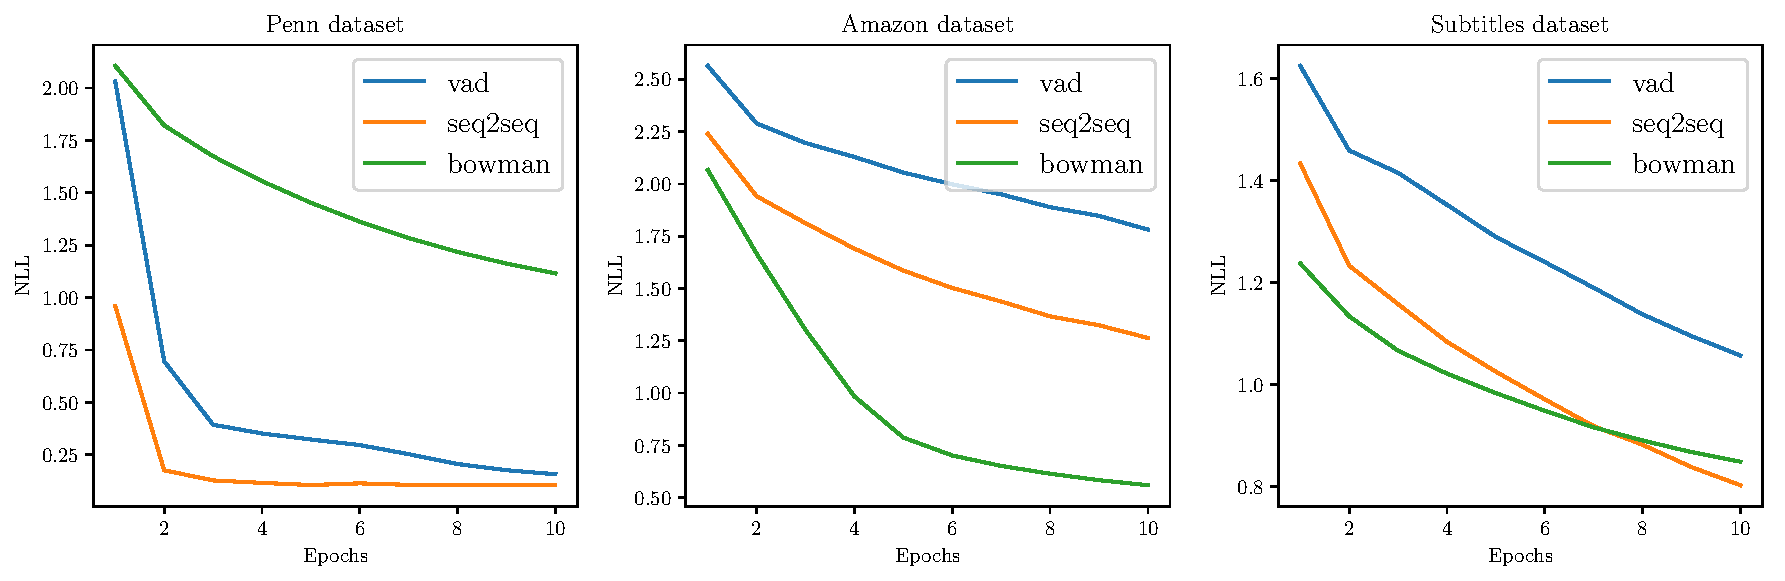
\includegraphics[width=150mm]{results/nll.pdf}
	\caption{Reconstruction losses of the three models across the three datasets; lower loss is better. \label{r:nll}}
  \end{figure}

% what is it? how is it measured? what does it say
With the Penn TreeBank dataset, The results shown are not particularly surprising. As there are less weights to learn, it was expected that Seq2Seq model would converge faster than the other models. Additionally, variational models are expected to perform worse than discrete models as the sampling mechanism will produce some variation in the responses. Interestingly the Bowman model performed the worst on the Penn dataset.

For the Amazon and Subtitles dataset, we observe that the Bowman model converges somewhat dubiously  quickly, but the other statistics show that the bowman model has understood little about the dataset. The VAD and Seq2Seq has performed within expectations in terms of relative learning.
% talk about the fact that this is not a good start anyway

% \subsection{KL Loss}

% \begin{figure}[!ht]
% 	\centering
% 	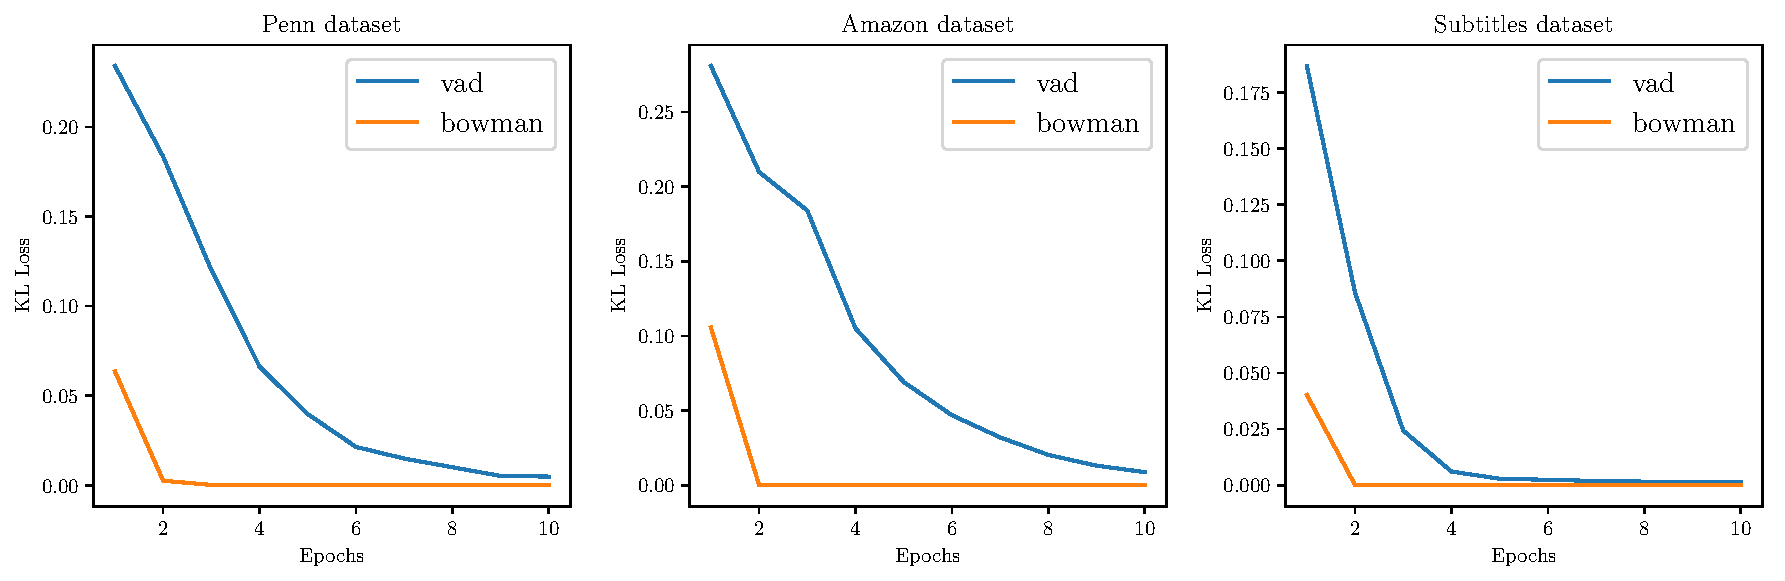
\includegraphics[width=150mm]{results/kl_loss.pdf}
% 	\caption{KL losses of the three models across the three datasets; higher is better.\label{r:kl_loss}}
% 	\end{figure}
	
% We measure the KL loss to determine the rate of which the amount of information is stored in the latent variable. Typically, we expect the models to produce some non-zero KL response, but we have noticed examples of KL collapse with the bowman approach. With the VAD, we observe larger KL values relative to the bowman model, suggesting that the auxiliary function works as intended for all types of datasets.

% In a similar fashion, the bowman model is expected to perform weaker than the VAD approach as the objective of the latent vector is to encompass properties of the data from a global sequence. 

\subsection{KL Ratio}

Interestingly, it was easier for the VAD to initially encode more information into the latent variable for the Penn dataset. It is suggested that it is probably the case that when comparing the overall ELBO loss, the VAD model has most likely overfit on the dataset; leading it to destroy any progress during learning.

\begin{figure}[!ht]
	\centering
	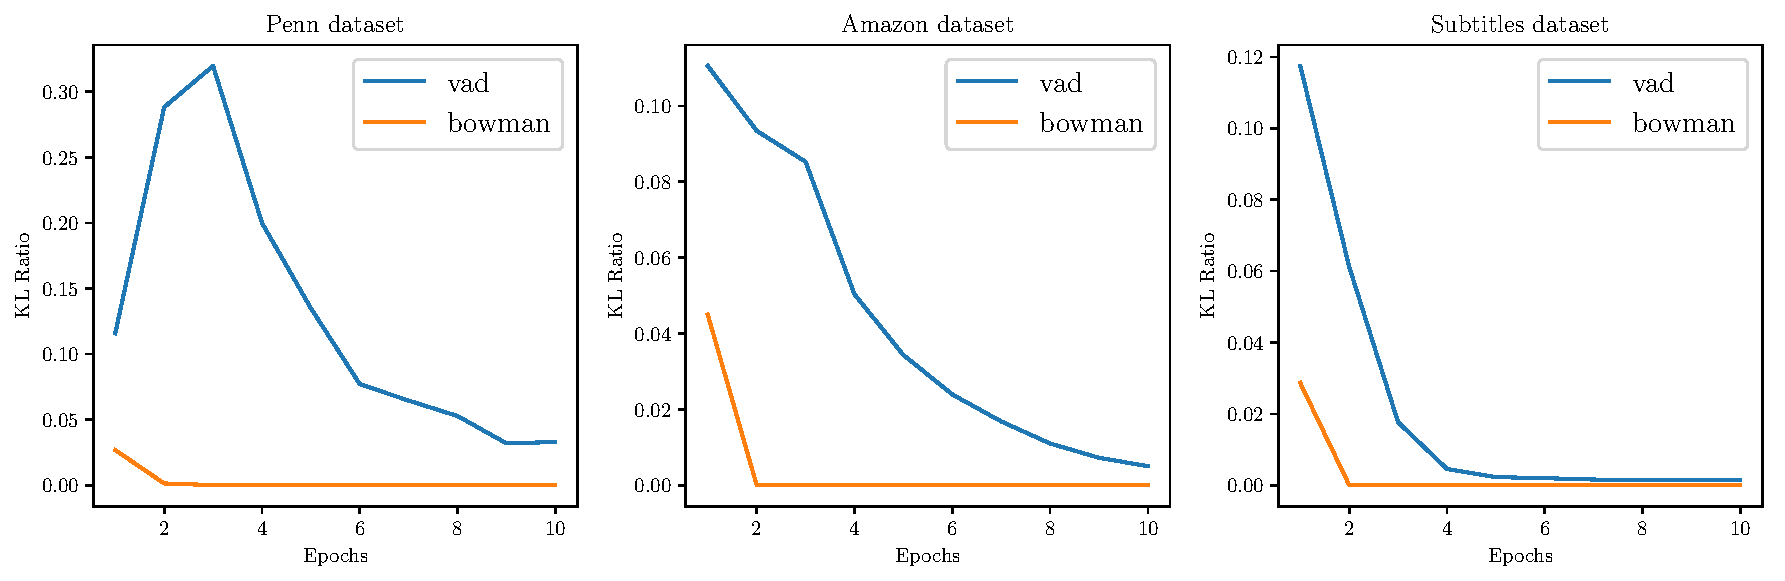
\includegraphics[width=150mm]{results/kl_ratio.pdf}
	\caption{KL ratios of the three models across the three datasets; higher is better.\label{r:kl_ratio}}
	\end{figure}

It however manages to encode some non-zero KL ratios on the other datasets, albeit it encompasses a small fraction of the ELBO. This could potentially be caused by the fact that the discourses in these datasets are one-to-many responses - The model may be confused by the various outcomes, forcing it to understand more on the reconstructive side as opposed to the variational sides.

\section{Linguistic Analysis}
Note that from this section onwards, we will be looking at the performance against the test splits of the datasets. 

\subsection{BLEU and ROUGE}
\begin{figure}[!ht]
	\centering
	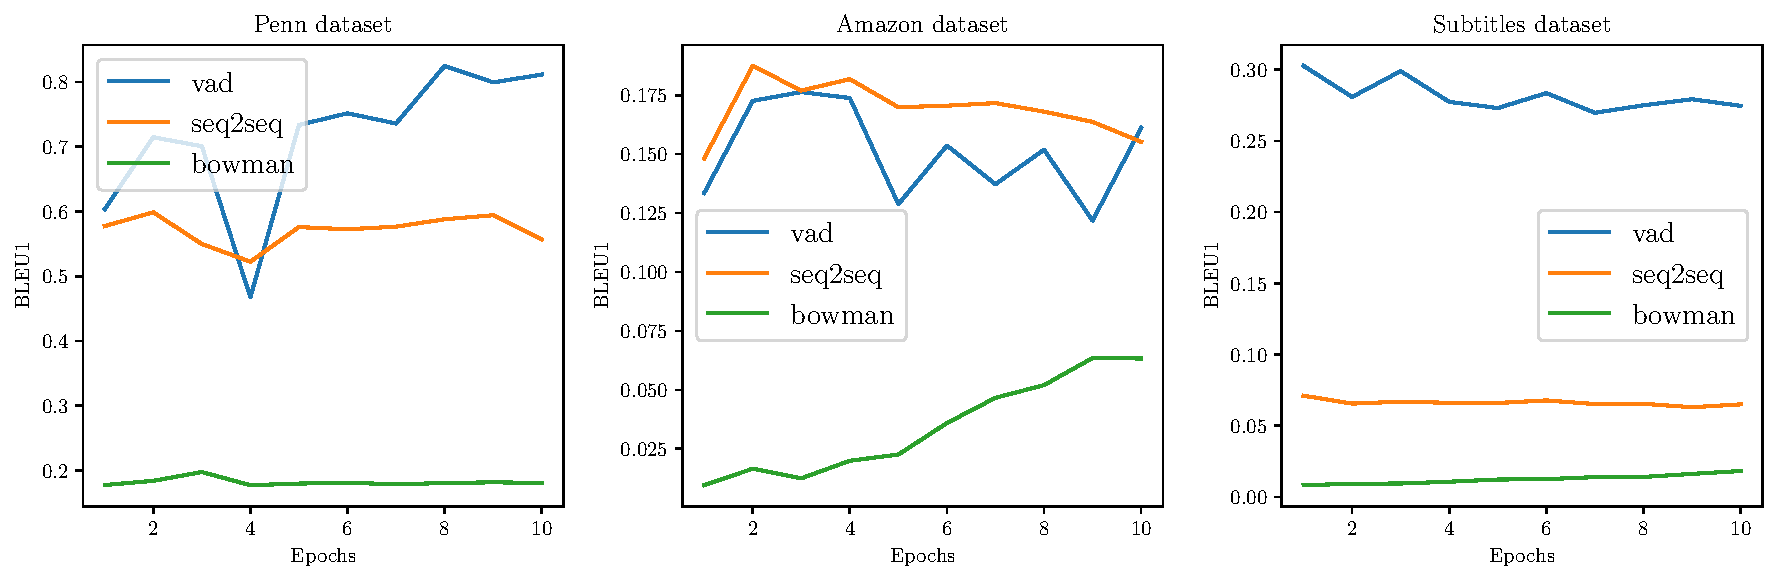
\includegraphics[width=150mm]{results/bleu1.pdf}
	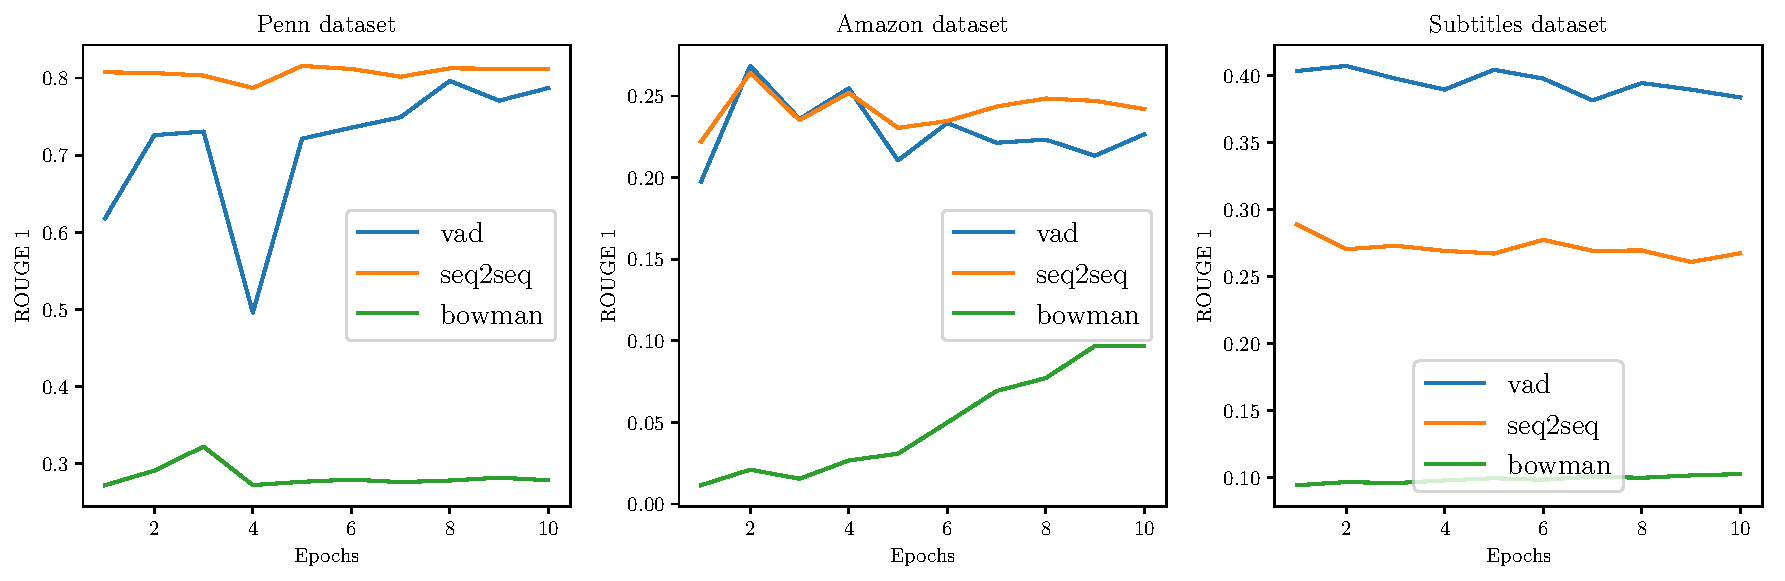
\includegraphics[width=150mm]{results/rouge_1.pdf}
	\caption{BLEU\textsubscript{1} (top) and ROUGE\textsubscript{1} (bottom) scores across the three models; higher is better.\label{r:bleu_rouge}}
  \end{figure}

Surprisingly, results for the Penn Dataset (Figure \ref{r:bleu_rouge}, left), the VAD is stronger than the other models by a considerable margin for both BLEU and ROUGE suggesting that it performs very strongly as an autoencoder. The VAD also performs considerably better on the Subtitles dataset  (Figure \ref{r:bleu_rouge}, right) against Seq2Seq, indicating its applicability for conditional response generation.

The VAD is somewhat comparable with Seq2Seq on the Amazon dataset  (Figure \ref{r:bleu_rouge}, center). This is somewhat contradictory to its performance on the Subtitles dataset, which may indicate some issue with how the Amazon dataset is initialised.

Unexpectedly the Bowman model performs considerably poorly against the Penn Dataset. Under further investigation with the Sampling examples, we see that the Bowman model does indeed capture the high level features, but the outputs do not reflect that of the input. Attempts to verify the authenticity of the results also confirm this. \footnote{The Bowman Model was tested on a popular GitHub implementation, which can be found on \href{https://github.com/timbmg/Sentence-VAE}{https://github.com/timbmg/Sentence-VAE.}
} For the other datasets, it was expected that this model would perform poorly by design, for reasons stated earlier (see Section \ref{variational_context}). 

\subsection{F1}

\begin{figure}[!ht]
	\centering
	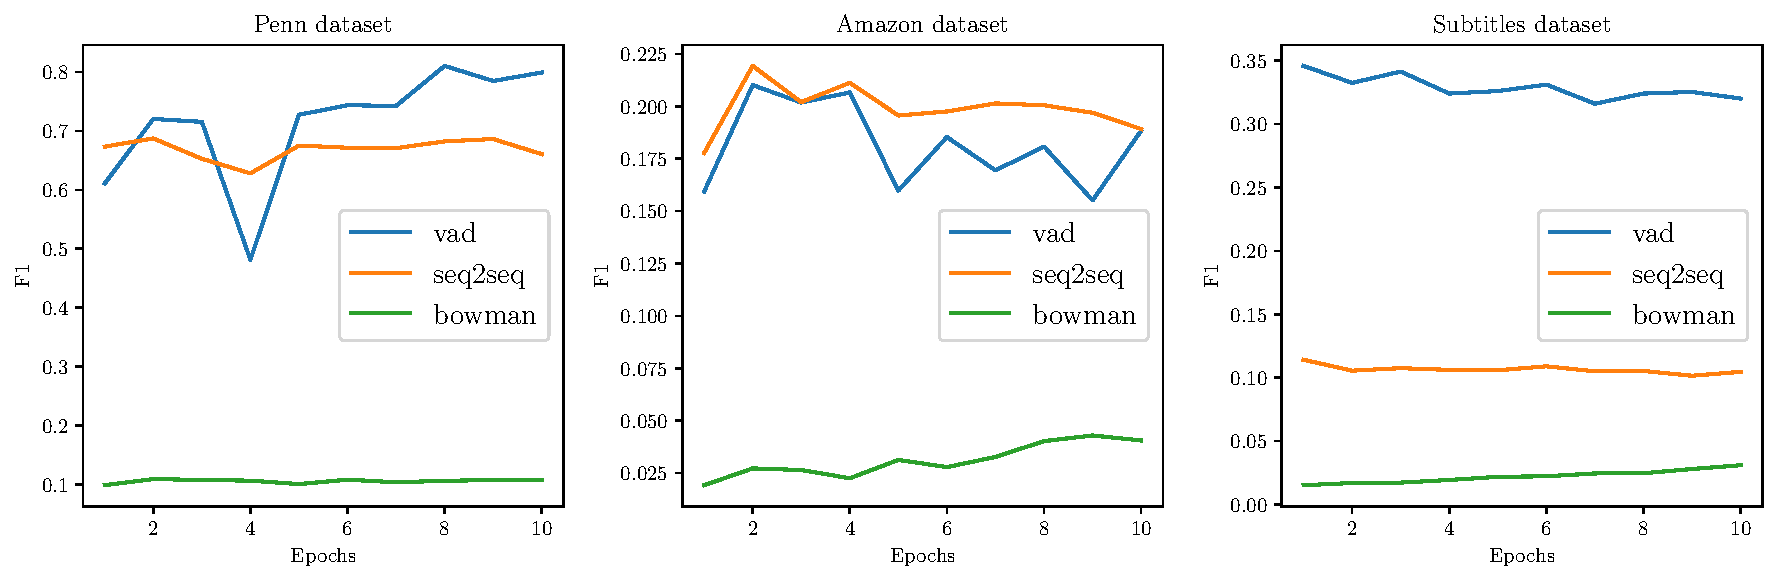
\includegraphics[width=150mm]{results/f1.pdf}
	\caption{F1\textsubscript{1-gram} scores across the three models; higher is better.\label{r:f1}}
	\end{figure}
	
The VAD performs the best with the Penn and Subtitles dataset, and is tied for the Amazon dataset. This strikes as particularly interesting, as it was originally hypothesised that additional conditional information could have helped to guide the responses.

Interestingly, the conditional datasets (Amazon and Subtitles) seem somewhat punishing for the models, with objectively low F1 scores. When compared to the example responses in Section \label{sampling_examples}, we notice that the responses are somewhat related and coherent for the VAD and Seq2Seq. One possible reason for is due to the open-endedness of responses in both of these datasets, where some fixed dialogue may typically lead to multiple responses\footnote{e.g. With the Subtitles dataset, a query with "who is it?" could elicit a variety of responses.}.

% what is it? how is it measured? what does it say

\subsection{Output Variance}

\begin{figure}[!ht]
	\centering
	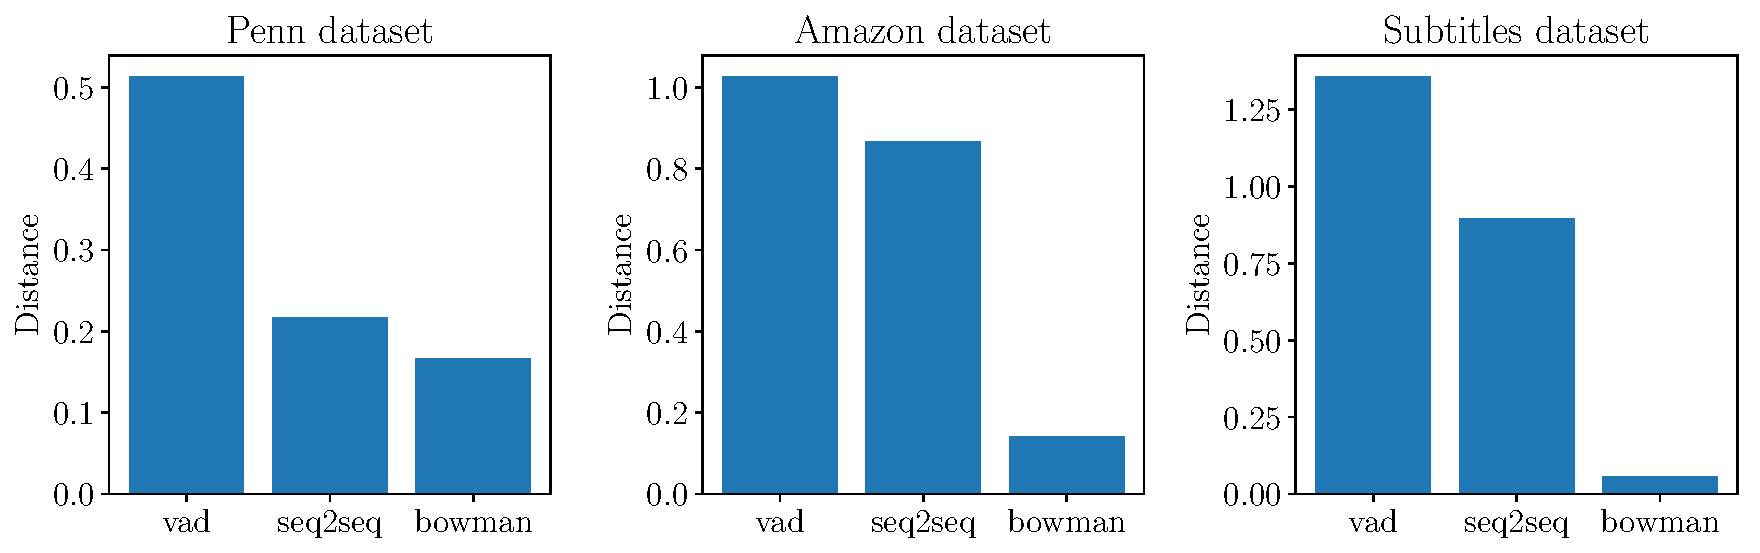
\includegraphics[width=150mm]{results/semantic_similarity.pdf}
	\caption{Semantic similarity scores across the datasets and models, higher is better.\label{r:variance}}
	\end{figure}

We can clearly see the disparity of the results between the models, with the VAD performing the best across the datasets. High variance for the Seq2Seq model on the Amazon and Subtitles dataset puts more confidence on the suggestion made earlier about one-to-many responses. 

The Penn dataset represents a case where the latent sampling comes into play and shows a scenario it does increase the variance in the results, for the Bowman model. Otherwise, for the other datasets, the Bowman model naturally underperforms and leaves much to be desired.

\subsection{Sampling Examples}
\label{sampling_examples}
Table \ref{qualitative_table} shows some of the outputs generated from the three models, against the three datasets. As some of our models are based on bayesian inference, we sample ten outputs and hand pick the most interesting responses from the datasets from each of the relevant models. 

\begin{table}[!ht]
	\centering
	\footnotesize
	\begin{tabular}{|p{1.5cm}|p{2.8cm}|p{2.8cm}|p{2.8cm}|p{2.8cm}|}
		\hline
		\textbf{Dataset}       & \textbf{Query}                                                                                                                                & \textbf{Bowman}                                           & \textbf{Seq2Seq}                                                   & \textbf{VAD}                                                               \\ \hline
		\textbf{Penn}          & these stocks eventually reopened                                                                                                              & the  \textless{}unk\textgreater\space \$ cents \textless{}unk\textgreater\space the \textless{}unk\textgreater\space  open                   & these stocks eventually reopened                                   & these stocks eventually reopened                                           \\ \cline{2-5} 
													 & as a result the link between the futures and stock markets , apart                                                                            & they is n't elaborate whether the \textless{}unk\textgreater\space  is a we is s going to be a a years & as a result the link between the futures and stock markets , apart & as a result the link between the futures between and futures markets apart \\ \hline
		\textbf{Open Subtitles} & i give you ride .                                                                                                                             & N/A                                                       & you ' re going to take a delivery hour                             & i ' m gon na take a walk .                                                 \\ \cline{2-5} 
													 & not exactly .                                                                                                                                 & ?                                                         & he ' s hideous \textless{}unk\textgreater , he ' s a musician      & i ' m gon na be able to finish the door .                                  \\ \hline
		\textbf{Amazon}        & b 0 0 d q d c 1 y 6 rating\_4.0 polarity\_0.8 i also have a background in it .                                                                & i the : the the the , you 's the i , is the ,             & i am going to get it to work well .                                & the email has a nice connection .                                          \\ \cline{2-5} 
													 & b 0 0 9 l l 9 v d g rating\_5.0 polarity\_-0.8 you will need the desktop to run larger things off of , and to use a printer remotely . & N/A                                                       & i have a fit of the canon .                                        & i a little to in distracting for the price .                               \\ \hline
	\end{tabular}
	\caption{Responses generated from the models across the datasets.}
	\label{qualitative_table}
\end{table}

For the Subtitles dataset, it was observed that the VAD generated linguistically superior and more plausible results compared to the Seq2Seq network. These results compliment the quantitative measurements observed earlier.

On the contrary, all models performed less admirably on the Amazon dataset. The Seq2Seq and VAD model produces somewhat coherent responses but generates relatively generic responses, or does not leverage the contexts provided by the query enough.

The Bowman model failed to generate remotely coherent responses for the Open Subtitles and Amazon datasets, and this is most likely related to the fact that it was designed for representation learning.

\chapter{Evaluation and Future Work}

Although some of the datasets were different and varying in purpose, scores are weaker for all models compared to their portrayed potential in their respective papers. This could primarily be attributed to two causes: (1) The dataset sizes used for the models were too small (as they were reduced to accomodate feasible training times), or (2) hyperparameter optimisation was too short in duration. In hindsight, increasing both should provide a clearer potential performance across the models, but the timescale and computational resources for the project was limited and could not afford the ability to scale up.

Further work should be taken to understand the influence of the BOW loss. Attempts to contact the the authors of the VAD paper have been unsuccessful, and it remains unclear what the influence of the $\alpha$ is in regards to the weight of the BOW loss. Initial experiments have shown a positive correlation with the KL divergence when $\alpha$ is increased, but details remain uncertain. An assorted set of additional comments are below:

\begin{itemize}  
\item Generated responses may not necessarily be indicative of the data it is modelled against.
\item Although there are mechanisms to control the vanishing KL problem, it is yet to be seen how universally applicable it would be.
\item The amount of hyperparameter tuning for the VAD is considerably larger than other neural models due to the inclusion of additional mechanisms for controlling the vanishing KL.
\item Further testing of the additional components introduced to the VAE should be measured independently to measure their influence to the KL loss. 
\item BLEU/ROUGE calculations should have been taken on the best output instead of an average of the whole sequence, but required extensive memory usage and would take a considerably longer running time due to technical implementation. In hindsight, this should have been considered as an additional measurement to improve the robustness of the results.
\item The Amazon reviews sequence data could have more experimentation. For instance, the ISIN/Item ID could be represented as a single word token as opposed to broken down by character level, and the  embedding value could be the mean of the embedding values of the character level tokens. Alternatively, the item identities could be inserted into the model through another input to the decoder, as opposed to concatenating it onto the input sequence. 
\item There is a potential for improving the KL performance by masking the SBOW matrix to the predicted output, such that the reconstruction loss would be a directly influenced by the auxiliary function.
\item An additional measurement could be used to determine whether the language models could pass off as a replacement to the original dataset. A classification model could be used to segregate sentences between the dataset and model generated samples. 
\end{itemize}


\begingroup
\renewcommand{\cleardoublepage}{}
\renewcommand{\clearpage}{}
\chapter{Conclusion}
\endgroup

In conclusion, we explored a neural language model in detail that could potentially be used for the purposes of encompassing the lexical variety of the original dataset. We have discussed the limitations of the model and used them to augment the components in a manner that allows them to work in unison. By subjecting them to quantitative and qualitative experimental results, we discover that the VAD can be sensibly considered for the task at hand. In future works, the model could be extended such that it would produce stronger and more lexically coherent discourses in a similar fashion as the dataset. One particularly interesting avenue for exploration could be related to adversarial approaches, which could be used in unison with the model to improve the diversity of artificial text generation.

\bibliographystyle{apa}
\begin{small}
\bibliography{ref} 
\end{small}
\chapter{Appendix}

\section{KL Divergence Derivation}
\label{kl_derivation}
Let $\mu_1, \sigma_1 \rightarrow \mathcal{N}(\mu_1,\sigma_1)$ be our first distribution, and $\mu_2, \sigma_2 \rightarrow \mathcal{N}(\mu_2,\sigma_2)$ be our second distribution. By deriving this, we would be able to calculate a derivative friendly loss function for our models.

\begin{equation}
	\label{eq:t}
	\begin{aligned}
	KL &= \int \left[\log( p(x)) - \log( q(x)) \right]\ p(x)\ dx \\
	% &= \frac{1}{2}\left[\log\frac{|\Sigma_2|}{|\Sigma_1|} - d + tr(\Sigma_2^{-1}\Sigma_1) + (\mu_2 - \mu_1)^T \Sigma_2^{-1}(\mu_2 - \mu_1)\right] \\
	&= \int \left[ \frac{1}{2} \log\frac{|\Sigma_2|}{|\Sigma_1|} - \frac{1}{2} (x-\mu_1)^T\Sigma_1^{-1}(x-\mu_1) + \frac{1}{2} (x-\mu_2)^T\Sigma_2^{-1}(x-\mu_2) \right] \times p(x) dx \\
	&= \frac{1}{2} \log\frac{|\Sigma_2|}{|\Sigma_1|} - \frac{1}{2} \text{tr}\ \left\{E[(x - \mu_1)(x - \mu_1)^T] \ \Sigma_1^{-1} \right\} + \frac{1}{2} E[(x - \mu_2)^T \Sigma_2^{-1} (x - \mu_2)] \\
	&= \frac{1}{2} \log\frac{|\Sigma_2|}{|\Sigma_1|} - \frac{1}{2} \text{tr}\ \{I_d \} + \frac{1}{2} (\mu_1 - \mu_2)^T \Sigma_2^{-1} (\mu_1 - \mu_2) + \frac{1}{2} \text{tr} \{ \Sigma_2^{-1} \Sigma_1 \} \\
	&= \frac{1}{2}\left[\log\frac{|\Sigma_2|}{|\Sigma_1|} - d + \text{tr} \{ \Sigma_2^{-1}\Sigma_1 \} + (\mu_2 - \mu_1)^T \Sigma_2^{-1}(\mu_2 - \mu_1)\right].
\end{aligned}
\end{equation}

\end{document}
